
\documentclass{article}

\usepackage{microtype}
\usepackage{graphicx}
\usepackage{subfigure}
\usepackage{booktabs} %


\usepackage{hyperref}

\newcommand{\theHalgorithm}{\arabic{algorithm}}

\usepackage[preprint]{icml2025}


\usepackage{amsmath}
\usepackage{amssymb}
\usepackage{mathtools}
\usepackage{amsthm}

\usepackage[capitalize, noabbrev]{cleveref}

\theoremstyle{plain}
\newtheorem{theorem}{Theorem}[section]
\newtheorem{proposition}[theorem]{Proposition}
\newtheorem{lemma}[theorem]{Lemma}
\newtheorem{corollary}[theorem]{Corollary}
\theoremstyle{definition}
\newtheorem{definition}[theorem]{Definition}
\newtheorem{assumption}[theorem]{Assumption}
\theoremstyle{remark}
\newtheorem{remark}[theorem]{Remark}

\usepackage[textsize=tiny]{todonotes}

\usepackage{multirow}
%%%%% NEW MATH DEFINITIONS %%%%%

\usepackage{amsmath,amsfonts,bm}
\usepackage{derivative}
% Mark sections of captions for referring to divisions of figures
\newcommand{\figleft}{{\em (Left)}}
\newcommand{\figcenter}{{\em (Center)}}
\newcommand{\figright}{{\em (Right)}}
\newcommand{\figtop}{{\em (Top)}}
\newcommand{\figbottom}{{\em (Bottom)}}
\newcommand{\captiona}{{\em (a)}}
\newcommand{\captionb}{{\em (b)}}
\newcommand{\captionc}{{\em (c)}}
\newcommand{\captiond}{{\em (d)}}

% Highlight a newly defined term
\newcommand{\newterm}[1]{{\bf #1}}

% Derivative d 
\newcommand{\deriv}{{\mathrm{d}}}

% Figure reference, lower-case.
\def\figref#1{figure~\ref{#1}}
% Figure reference, capital. For start of sentence
\def\Figref#1{Figure~\ref{#1}}
\def\twofigref#1#2{figures \ref{#1} and \ref{#2}}
\def\quadfigref#1#2#3#4{figures \ref{#1}, \ref{#2}, \ref{#3} and \ref{#4}}
% Section reference, lower-case.
\def\secref#1{section~\ref{#1}}
% Section reference, capital.
\def\Secref#1{Section~\ref{#1}}
% Reference to two sections.
\def\twosecrefs#1#2{sections \ref{#1} and \ref{#2}}
% Reference to three sections.
\def\secrefs#1#2#3{sections \ref{#1}, \ref{#2} and \ref{#3}}
% Reference to an equation, lower-case.
\def\eqref#1{equation~\ref{#1}}
% Reference to an equation, upper case
\def\Eqref#1{Equation~\ref{#1}}
% A raw reference to an equation---avoid using if possible
\def\plaineqref#1{\ref{#1}}
% Reference to a chapter, lower-case.
\def\chapref#1{chapter~\ref{#1}}
% Reference to an equation, upper case.
\def\Chapref#1{Chapter~\ref{#1}}
% Reference to a range of chapters
\def\rangechapref#1#2{chapters\ref{#1}--\ref{#2}}
% Reference to an algorithm, lower-case.
\def\algref#1{algorithm~\ref{#1}}
% Reference to an algorithm, upper case.
\def\Algref#1{Algorithm~\ref{#1}}
\def\twoalgref#1#2{algorithms \ref{#1} and \ref{#2}}
\def\Twoalgref#1#2{Algorithms \ref{#1} and \ref{#2}}
% Reference to a part, lower case
\def\partref#1{part~\ref{#1}}
% Reference to a part, upper case
\def\Partref#1{Part~\ref{#1}}
\def\twopartref#1#2{parts \ref{#1} and \ref{#2}}

\def\ceil#1{\lceil #1 \rceil}
\def\floor#1{\lfloor #1 \rfloor}
\def\1{\bm{1}}
\newcommand{\train}{\mathcal{D}}
\newcommand{\valid}{\mathcal{D_{\mathrm{valid}}}}
\newcommand{\test}{\mathcal{D_{\mathrm{test}}}}

\def\eps{{\epsilon}}


% Random variables
\def\reta{{\textnormal{$\eta$}}}
\def\ra{{\textnormal{a}}}
\def\rb{{\textnormal{b}}}
\def\rc{{\textnormal{c}}}
\def\rd{{\textnormal{d}}}
\def\re{{\textnormal{e}}}
\def\rf{{\textnormal{f}}}
\def\rg{{\textnormal{g}}}
\def\rh{{\textnormal{h}}}
\def\ri{{\textnormal{i}}}
\def\rj{{\textnormal{j}}}
\def\rk{{\textnormal{k}}}
\def\rl{{\textnormal{l}}}
% rm is already a command, just don't name any random variables m
\def\rn{{\textnormal{n}}}
\def\ro{{\textnormal{o}}}
\def\rp{{\textnormal{p}}}
\def\rq{{\textnormal{q}}}
\def\rr{{\textnormal{r}}}
\def\rs{{\textnormal{s}}}
\def\rt{{\textnormal{t}}}
\def\ru{{\textnormal{u}}}
\def\rv{{\textnormal{v}}}
\def\rw{{\textnormal{w}}}
\def\rx{{\textnormal{x}}}
\def\ry{{\textnormal{y}}}
\def\rz{{\textnormal{z}}}

% Random vectors
\def\rvepsilon{{\mathbf{\epsilon}}}
\def\rvphi{{\mathbf{\phi}}}
\def\rvtheta{{\mathbf{\theta}}}
\def\rva{{\mathbf{a}}}
\def\rvb{{\mathbf{b}}}
\def\rvc{{\mathbf{c}}}
\def\rvd{{\mathbf{d}}}
\def\rve{{\mathbf{e}}}
\def\rvf{{\mathbf{f}}}
\def\rvg{{\mathbf{g}}}
\def\rvh{{\mathbf{h}}}
\def\rvu{{\mathbf{i}}}
\def\rvj{{\mathbf{j}}}
\def\rvk{{\mathbf{k}}}
\def\rvl{{\mathbf{l}}}
\def\rvm{{\mathbf{m}}}
\def\rvn{{\mathbf{n}}}
\def\rvo{{\mathbf{o}}}
\def\rvp{{\mathbf{p}}}
\def\rvq{{\mathbf{q}}}
\def\rvr{{\mathbf{r}}}
\def\rvs{{\mathbf{s}}}
\def\rvt{{\mathbf{t}}}
\def\rvu{{\mathbf{u}}}
\def\rvv{{\mathbf{v}}}
\def\rvw{{\mathbf{w}}}
\def\rvx{{\mathbf{x}}}
\def\rvy{{\mathbf{y}}}
\def\rvz{{\mathbf{z}}}

% Elements of random vectors
\def\erva{{\textnormal{a}}}
\def\ervb{{\textnormal{b}}}
\def\ervc{{\textnormal{c}}}
\def\ervd{{\textnormal{d}}}
\def\erve{{\textnormal{e}}}
\def\ervf{{\textnormal{f}}}
\def\ervg{{\textnormal{g}}}
\def\ervh{{\textnormal{h}}}
\def\ervi{{\textnormal{i}}}
\def\ervj{{\textnormal{j}}}
\def\ervk{{\textnormal{k}}}
\def\ervl{{\textnormal{l}}}
\def\ervm{{\textnormal{m}}}
\def\ervn{{\textnormal{n}}}
\def\ervo{{\textnormal{o}}}
\def\ervp{{\textnormal{p}}}
\def\ervq{{\textnormal{q}}}
\def\ervr{{\textnormal{r}}}
\def\ervs{{\textnormal{s}}}
\def\ervt{{\textnormal{t}}}
\def\ervu{{\textnormal{u}}}
\def\ervv{{\textnormal{v}}}
\def\ervw{{\textnormal{w}}}
\def\ervx{{\textnormal{x}}}
\def\ervy{{\textnormal{y}}}
\def\ervz{{\textnormal{z}}}

% Random matrices
\def\rmA{{\mathbf{A}}}
\def\rmB{{\mathbf{B}}}
\def\rmC{{\mathbf{C}}}
\def\rmD{{\mathbf{D}}}
\def\rmE{{\mathbf{E}}}
\def\rmF{{\mathbf{F}}}
\def\rmG{{\mathbf{G}}}
\def\rmH{{\mathbf{H}}}
\def\rmI{{\mathbf{I}}}
\def\rmJ{{\mathbf{J}}}
\def\rmK{{\mathbf{K}}}
\def\rmL{{\mathbf{L}}}
\def\rmM{{\mathbf{M}}}
\def\rmN{{\mathbf{N}}}
\def\rmO{{\mathbf{O}}}
\def\rmP{{\mathbf{P}}}
\def\rmQ{{\mathbf{Q}}}
\def\rmR{{\mathbf{R}}}
\def\rmS{{\mathbf{S}}}
\def\rmT{{\mathbf{T}}}
\def\rmU{{\mathbf{U}}}
\def\rmV{{\mathbf{V}}}
\def\rmW{{\mathbf{W}}}
\def\rmX{{\mathbf{X}}}
\def\rmY{{\mathbf{Y}}}
\def\rmZ{{\mathbf{Z}}}

% Elements of random matrices
\def\ermA{{\textnormal{A}}}
\def\ermB{{\textnormal{B}}}
\def\ermC{{\textnormal{C}}}
\def\ermD{{\textnormal{D}}}
\def\ermE{{\textnormal{E}}}
\def\ermF{{\textnormal{F}}}
\def\ermG{{\textnormal{G}}}
\def\ermH{{\textnormal{H}}}
\def\ermI{{\textnormal{I}}}
\def\ermJ{{\textnormal{J}}}
\def\ermK{{\textnormal{K}}}
\def\ermL{{\textnormal{L}}}
\def\ermM{{\textnormal{M}}}
\def\ermN{{\textnormal{N}}}
\def\ermO{{\textnormal{O}}}
\def\ermP{{\textnormal{P}}}
\def\ermQ{{\textnormal{Q}}}
\def\ermR{{\textnormal{R}}}
\def\ermS{{\textnormal{S}}}
\def\ermT{{\textnormal{T}}}
\def\ermU{{\textnormal{U}}}
\def\ermV{{\textnormal{V}}}
\def\ermW{{\textnormal{W}}}
\def\ermX{{\textnormal{X}}}
\def\ermY{{\textnormal{Y}}}
\def\ermZ{{\textnormal{Z}}}

% Vectors
\def\vzero{{\bm{0}}}
\def\vone{{\bm{1}}}
\def\vmu{{\bm{\mu}}}
\def\vtheta{{\bm{\theta}}}
\def\vphi{{\bm{\phi}}}
\def\va{{\bm{a}}}
\def\vb{{\bm{b}}}
\def\vc{{\bm{c}}}
\def\vd{{\bm{d}}}
\def\ve{{\bm{e}}}
\def\vf{{\bm{f}}}
\def\vg{{\bm{g}}}
\def\vh{{\bm{h}}}
\def\vi{{\bm{i}}}
\def\vj{{\bm{j}}}
\def\vk{{\bm{k}}}
\def\vl{{\bm{l}}}
\def\vm{{\bm{m}}}
\def\vn{{\bm{n}}}
\def\vo{{\bm{o}}}
\def\vp{{\bm{p}}}
\def\vq{{\bm{q}}}
\def\vr{{\bm{r}}}
\def\vs{{\bm{s}}}
\def\vt{{\bm{t}}}
\def\vu{{\bm{u}}}
\def\vv{{\bm{v}}}
\def\vw{{\bm{w}}}
\def\vx{{\bm{x}}}
\def\vy{{\bm{y}}}
\def\vz{{\bm{z}}}

% Elements of vectors
\def\evalpha{{\alpha}}
\def\evbeta{{\beta}}
\def\evepsilon{{\epsilon}}
\def\evlambda{{\lambda}}
\def\evomega{{\omega}}
\def\evmu{{\mu}}
\def\evpsi{{\psi}}
\def\evsigma{{\sigma}}
\def\evtheta{{\theta}}
\def\eva{{a}}
\def\evb{{b}}
\def\evc{{c}}
\def\evd{{d}}
\def\eve{{e}}
\def\evf{{f}}
\def\evg{{g}}
\def\evh{{h}}
\def\evi{{i}}
\def\evj{{j}}
\def\evk{{k}}
\def\evl{{l}}
\def\evm{{m}}
\def\evn{{n}}
\def\evo{{o}}
\def\evp{{p}}
\def\evq{{q}}
\def\evr{{r}}
\def\evs{{s}}
\def\evt{{t}}
\def\evu{{u}}
\def\evv{{v}}
\def\evw{{w}}
\def\evx{{x}}
\def\evy{{y}}
\def\evz{{z}}

% Matrix
\def\mA{{\bm{A}}}
\def\mB{{\bm{B}}}
\def\mC{{\bm{C}}}
\def\mD{{\bm{D}}}
\def\mE{{\bm{E}}}
\def\mF{{\bm{F}}}
\def\mG{{\bm{G}}}
\def\mH{{\bm{H}}}
\def\mI{{\bm{I}}}
\def\mJ{{\bm{J}}}
\def\mK{{\bm{K}}}
\def\mL{{\bm{L}}}
\def\mM{{\bm{M}}}
\def\mN{{\bm{N}}}
\def\mO{{\bm{O}}}
\def\mP{{\bm{P}}}
\def\mQ{{\bm{Q}}}
\def\mR{{\bm{R}}}
\def\mS{{\bm{S}}}
\def\mT{{\bm{T}}}
\def\mU{{\bm{U}}}
\def\mV{{\bm{V}}}
\def\mW{{\bm{W}}}
\def\mX{{\bm{X}}}
\def\mY{{\bm{Y}}}
\def\mZ{{\bm{Z}}}
\def\mBeta{{\bm{\beta}}}
\def\mPhi{{\bm{\Phi}}}
\def\mLambda{{\bm{\Lambda}}}
\def\mSigma{{\bm{\Sigma}}}

% Tensor
\DeclareMathAlphabet{\mathsfit}{\encodingdefault}{\sfdefault}{m}{sl}
\SetMathAlphabet{\mathsfit}{bold}{\encodingdefault}{\sfdefault}{bx}{n}
\newcommand{\tens}[1]{\bm{\mathsfit{#1}}}
\def\tA{{\tens{A}}}
\def\tB{{\tens{B}}}
\def\tC{{\tens{C}}}
\def\tD{{\tens{D}}}
\def\tE{{\tens{E}}}
\def\tF{{\tens{F}}}
\def\tG{{\tens{G}}}
\def\tH{{\tens{H}}}
\def\tI{{\tens{I}}}
\def\tJ{{\tens{J}}}
\def\tK{{\tens{K}}}
\def\tL{{\tens{L}}}
\def\tM{{\tens{M}}}
\def\tN{{\tens{N}}}
\def\tO{{\tens{O}}}
\def\tP{{\tens{P}}}
\def\tQ{{\tens{Q}}}
\def\tR{{\tens{R}}}
\def\tS{{\tens{S}}}
\def\tT{{\tens{T}}}
\def\tU{{\tens{U}}}
\def\tV{{\tens{V}}}
\def\tW{{\tens{W}}}
\def\tX{{\tens{X}}}
\def\tY{{\tens{Y}}}
\def\tZ{{\tens{Z}}}


% Graph
\def\gA{{\mathcal{A}}}
\def\gB{{\mathcal{B}}}
\def\gC{{\mathcal{C}}}
\def\gD{{\mathcal{D}}}
\def\gE{{\mathcal{E}}}
\def\gF{{\mathcal{F}}}
\def\gG{{\mathcal{G}}}
\def\gH{{\mathcal{H}}}
\def\gI{{\mathcal{I}}}
\def\gJ{{\mathcal{J}}}
\def\gK{{\mathcal{K}}}
\def\gL{{\mathcal{L}}}
\def\gM{{\mathcal{M}}}
\def\gN{{\mathcal{N}}}
\def\gO{{\mathcal{O}}}
\def\gP{{\mathcal{P}}}
\def\gQ{{\mathcal{Q}}}
\def\gR{{\mathcal{R}}}
\def\gS{{\mathcal{S}}}
\def\gT{{\mathcal{T}}}
\def\gU{{\mathcal{U}}}
\def\gV{{\mathcal{V}}}
\def\gW{{\mathcal{W}}}
\def\gX{{\mathcal{X}}}
\def\gY{{\mathcal{Y}}}
\def\gZ{{\mathcal{Z}}}

% Sets
\def\sA{{\mathbb{A}}}
\def\sB{{\mathbb{B}}}
\def\sC{{\mathbb{C}}}
\def\sD{{\mathbb{D}}}
% Don't use a set called E, because this would be the same as our symbol
% for expectation.
\def\sF{{\mathbb{F}}}
\def\sG{{\mathbb{G}}}
\def\sH{{\mathbb{H}}}
\def\sI{{\mathbb{I}}}
\def\sJ{{\mathbb{J}}}
\def\sK{{\mathbb{K}}}
\def\sL{{\mathbb{L}}}
\def\sM{{\mathbb{M}}}
\def\sN{{\mathbb{N}}}
\def\sO{{\mathbb{O}}}
\def\sP{{\mathbb{P}}}
\def\sQ{{\mathbb{Q}}}
\def\sR{{\mathbb{R}}}
\def\sS{{\mathbb{S}}}
\def\sT{{\mathbb{T}}}
\def\sU{{\mathbb{U}}}
\def\sV{{\mathbb{V}}}
\def\sW{{\mathbb{W}}}
\def\sX{{\mathbb{X}}}
\def\sY{{\mathbb{Y}}}
\def\sZ{{\mathbb{Z}}}

% Entries of a matrix
\def\emLambda{{\Lambda}}
\def\emA{{A}}
\def\emB{{B}}
\def\emC{{C}}
\def\emD{{D}}
\def\emE{{E}}
\def\emF{{F}}
\def\emG{{G}}
\def\emH{{H}}
\def\emI{{I}}
\def\emJ{{J}}
\def\emK{{K}}
\def\emL{{L}}
\def\emM{{M}}
\def\emN{{N}}
\def\emO{{O}}
\def\emP{{P}}
\def\emQ{{Q}}
\def\emR{{R}}
\def\emS{{S}}
\def\emT{{T}}
\def\emU{{U}}
\def\emV{{V}}
\def\emW{{W}}
\def\emX{{X}}
\def\emY{{Y}}
\def\emZ{{Z}}
\def\emSigma{{\Sigma}}

% entries of a tensor
% Same font as tensor, without \bm wrapper
\newcommand{\etens}[1]{\mathsfit{#1}}
\def\etLambda{{\etens{\Lambda}}}
\def\etA{{\etens{A}}}
\def\etB{{\etens{B}}}
\def\etC{{\etens{C}}}
\def\etD{{\etens{D}}}
\def\etE{{\etens{E}}}
\def\etF{{\etens{F}}}
\def\etG{{\etens{G}}}
\def\etH{{\etens{H}}}
\def\etI{{\etens{I}}}
\def\etJ{{\etens{J}}}
\def\etK{{\etens{K}}}
\def\etL{{\etens{L}}}
\def\etM{{\etens{M}}}
\def\etN{{\etens{N}}}
\def\etO{{\etens{O}}}
\def\etP{{\etens{P}}}
\def\etQ{{\etens{Q}}}
\def\etR{{\etens{R}}}
\def\etS{{\etens{S}}}
\def\etT{{\etens{T}}}
\def\etU{{\etens{U}}}
\def\etV{{\etens{V}}}
\def\etW{{\etens{W}}}
\def\etX{{\etens{X}}}
\def\etY{{\etens{Y}}}
\def\etZ{{\etens{Z}}}

% The true underlying data generating distribution
\newcommand{\pdata}{p_{\rm{data}}}
\newcommand{\ptarget}{p_{\rm{target}}}
\newcommand{\pprior}{p_{\rm{prior}}}
\newcommand{\pbase}{p_{\rm{base}}}
\newcommand{\pref}{p_{\rm{ref}}}

% The empirical distribution defined by the training set
\newcommand{\ptrain}{\hat{p}_{\rm{data}}}
\newcommand{\Ptrain}{\hat{P}_{\rm{data}}}
% The model distribution
\newcommand{\pmodel}{p_{\rm{model}}}
\newcommand{\Pmodel}{P_{\rm{model}}}
\newcommand{\ptildemodel}{\tilde{p}_{\rm{model}}}
% Stochastic autoencoder distributions
\newcommand{\pencode}{p_{\rm{encoder}}}
\newcommand{\pdecode}{p_{\rm{decoder}}}
\newcommand{\precons}{p_{\rm{reconstruct}}}

\newcommand{\laplace}{\mathrm{Laplace}} % Laplace distribution

\newcommand{\E}{\mathbb{E}}
\newcommand{\Ls}{\mathcal{L}}
\newcommand{\R}{\mathbb{R}}
\newcommand{\emp}{\tilde{p}}
\newcommand{\lr}{\alpha}
\newcommand{\reg}{\lambda}
\newcommand{\rect}{\mathrm{rectifier}}
\newcommand{\softmax}{\mathrm{softmax}}
\newcommand{\sigmoid}{\sigma}
\newcommand{\softplus}{\zeta}
\newcommand{\KL}{D_{\mathrm{KL}}}
\newcommand{\Var}{\mathrm{Var}}
\newcommand{\standarderror}{\mathrm{SE}}
\newcommand{\Cov}{\mathrm{Cov}}
% Wolfram Mathworld says $L^2$ is for function spaces and $\ell^2$ is for vectors
% But then they seem to use $L^2$ for vectors throughout the site, and so does
% wikipedia.
\newcommand{\normlzero}{L^0}
\newcommand{\normlone}{L^1}
\newcommand{\normltwo}{L^2}
\newcommand{\normlp}{L^p}
\newcommand{\normmax}{L^\infty}

\newcommand{\parents}{Pa} % See usage in notation.tex. Chosen to match Daphne's book.

\DeclareMathOperator*{\argmax}{arg\,max}
\DeclareMathOperator*{\argmin}{arg\,min}

\DeclareMathOperator{\sign}{sign}
\DeclareMathOperator{\Tr}{Tr}
\let\ab\allowbreak

\definecolor{lightgray}{gray}{.95}
\definecolor{lightyellow}{rgb}{1.0, 1.0, 0.88}
\definecolor{whitesmoke}{rgb}{0.96, 0.96, 0.96}
\definecolor{lightcyan}{rgb}{0.88, 1.0, 1.0}
\usepackage{thmtools}
\newcommand{\jiazheng}[1]{\textcolor{red}{[Jiazheng: #1]}}
\usepackage{siunitx}
\usepackage{titletoc}

\usepackage{hyperref}
\definecolor{cvprblue}{rgb}{0.21,0.49,0.74}
\definecolor{citecolor}{HTML}{2980b9}
\definecolor{linkcolor}{HTML}{c0392b}
\hypersetup{
    colorlinks=true,
    linkcolor=linkcolor,
    citecolor=citecolor,     
    urlcolor=linkcolor,
}

\usepackage{lipsum}
\usepackage{tikz}
\usepackage{multicol}
\usepackage{pifont}

\usepackage[ruled,vlined]{algorithm2e}
\SetKw{KwInit}{Init:}
\usepackage{tcolorbox}
\tcbuselibrary{breakable}

\newtcolorbox{introbox}{colback=gray!10!white, colframe=gray!50!black, boxrule=0.5pt, arc=2pt, left=2pt, right=2pt, top=2pt, bottom=2pt, breakable, width=\linewidth}
\newtcolorbox{initbox}{colback=yellow!10!white, colframe=yellow!50!black, boxrule=0.5pt, arc=2pt, left=2pt, right=2pt, top=2pt, bottom=2pt, breakable, width=\linewidth}
\newtcolorbox{optbox}{colback=blue!10!white, colframe=blue!50!black, boxrule=0.5pt, arc=2pt, left=2pt, right=2pt, top=2pt, bottom=2pt, breakable, width=0.933\linewidth}
\newtcolorbox{updatebox}{colback=green!10!white, colframe=green!50!black, boxrule=0.5pt, arc=2pt, left=2pt, right=2pt, top=2pt, bottom=2pt, breakable, width=0.866\linewidth}

\usepackage{enumitem}




\begin{document}
    \twocolumn[ \icmltitle{Scalable Model Merging with Progressive Layer-wise Distillation}




    \begin{icmlauthorlist}
        \icmlauthor{Jing Xu}{thu} 
        \icmlauthor{Jiazheng Li}{bit}
        \icmlauthor{Jingzhao Zhang}{thu,sqz}
    \end{icmlauthorlist}

    \icmlaffiliation{thu}{Institute for Interdisciplinary Information Sciences, Tsinghua University}
    \icmlaffiliation{bit}{School of Computer Science, Beijing Institute of Technology} 
    \icmlaffiliation{sqz}{Shanghai Qizhi Institute}

    \icmlcorrespondingauthor{Jing Xu}{xujing21@mails.tsinghua.edu.cn} 

    \icmlkeywords{Machine Learning, ICML}

    \vskip 0.3in ]



    \printAffiliationsAndNotice{}

    

    \begin{abstract}  
Test time scaling is currently one of the most active research areas that shows promise after training time scaling has reached its limits.
Deep-thinking (DT) models are a class of recurrent models that can perform easy-to-hard generalization by assigning more compute to harder test samples.
However, due to their inability to determine the complexity of a test sample, DT models have to use a large amount of computation for both easy and hard test samples.
Excessive test time computation is wasteful and can cause the ``overthinking'' problem where more test time computation leads to worse results.
In this paper, we introduce a test time training method for determining the optimal amount of computation needed for each sample during test time.
We also propose Conv-LiGRU, a novel recurrent architecture for efficient and robust visual reasoning. 
Extensive experiments demonstrate that Conv-LiGRU is more stable than DT, effectively mitigates the ``overthinking'' phenomenon, and achieves superior accuracy.
\end{abstract}  
    \section{Introduction}


\begin{figure}[t]
\centering
\includegraphics[width=0.6\columnwidth]{figures/evaluation_desiderata_V5.pdf}
\vspace{-0.5cm}
\caption{\systemName is a platform for conducting realistic evaluations of code LLMs, collecting human preferences of coding models with real users, real tasks, and in realistic environments, aimed at addressing the limitations of existing evaluations.
}
\label{fig:motivation}
\end{figure}

\begin{figure*}[t]
\centering
\includegraphics[width=\textwidth]{figures/system_design_v2.png}
\caption{We introduce \systemName, a VSCode extension to collect human preferences of code directly in a developer's IDE. \systemName enables developers to use code completions from various models. The system comprises a) the interface in the user's IDE which presents paired completions to users (left), b) a sampling strategy that picks model pairs to reduce latency (right, top), and c) a prompting scheme that allows diverse LLMs to perform code completions with high fidelity.
Users can select between the top completion (green box) using \texttt{tab} or the bottom completion (blue box) using \texttt{shift+tab}.}
\label{fig:overview}
\end{figure*}

As model capabilities improve, large language models (LLMs) are increasingly integrated into user environments and workflows.
For example, software developers code with AI in integrated developer environments (IDEs)~\citep{peng2023impact}, doctors rely on notes generated through ambient listening~\citep{oberst2024science}, and lawyers consider case evidence identified by electronic discovery systems~\citep{yang2024beyond}.
Increasing deployment of models in productivity tools demands evaluation that more closely reflects real-world circumstances~\citep{hutchinson2022evaluation, saxon2024benchmarks, kapoor2024ai}.
While newer benchmarks and live platforms incorporate human feedback to capture real-world usage, they almost exclusively focus on evaluating LLMs in chat conversations~\citep{zheng2023judging,dubois2023alpacafarm,chiang2024chatbot, kirk2024the}.
Model evaluation must move beyond chat-based interactions and into specialized user environments.



 

In this work, we focus on evaluating LLM-based coding assistants. 
Despite the popularity of these tools---millions of developers use Github Copilot~\citep{Copilot}---existing
evaluations of the coding capabilities of new models exhibit multiple limitations (Figure~\ref{fig:motivation}, bottom).
Traditional ML benchmarks evaluate LLM capabilities by measuring how well a model can complete static, interview-style coding tasks~\citep{chen2021evaluating,austin2021program,jain2024livecodebench, white2024livebench} and lack \emph{real users}. 
User studies recruit real users to evaluate the effectiveness of LLMs as coding assistants, but are often limited to simple programming tasks as opposed to \emph{real tasks}~\citep{vaithilingam2022expectation,ross2023programmer, mozannar2024realhumaneval}.
Recent efforts to collect human feedback such as Chatbot Arena~\citep{chiang2024chatbot} are still removed from a \emph{realistic environment}, resulting in users and data that deviate from typical software development processes.
We introduce \systemName to address these limitations (Figure~\ref{fig:motivation}, top), and we describe our three main contributions below.


\textbf{We deploy \systemName in-the-wild to collect human preferences on code.} 
\systemName is a Visual Studio Code extension, collecting preferences directly in a developer's IDE within their actual workflow (Figure~\ref{fig:overview}).
\systemName provides developers with code completions, akin to the type of support provided by Github Copilot~\citep{Copilot}. 
Over the past 3 months, \systemName has served over~\completions suggestions from 10 state-of-the-art LLMs, 
gathering \sampleCount~votes from \userCount~users.
To collect user preferences,
\systemName presents a novel interface that shows users paired code completions from two different LLMs, which are determined based on a sampling strategy that aims to 
mitigate latency while preserving coverage across model comparisons.
Additionally, we devise a prompting scheme that allows a diverse set of models to perform code completions with high fidelity.
See Section~\ref{sec:system} and Section~\ref{sec:deployment} for details about system design and deployment respectively.



\textbf{We construct a leaderboard of user preferences and find notable differences from existing static benchmarks and human preference leaderboards.}
In general, we observe that smaller models seem to overperform in static benchmarks compared to our leaderboard, while performance among larger models is mixed (Section~\ref{sec:leaderboard_calculation}).
We attribute these differences to the fact that \systemName is exposed to users and tasks that differ drastically from code evaluations in the past. 
Our data spans 103 programming languages and 24 natural languages as well as a variety of real-world applications and code structures, while static benchmarks tend to focus on a specific programming and natural language and task (e.g. coding competition problems).
Additionally, while all of \systemName interactions contain code contexts and the majority involve infilling tasks, a much smaller fraction of Chatbot Arena's coding tasks contain code context, with infilling tasks appearing even more rarely. 
We analyze our data in depth in Section~\ref{subsec:comparison}.



\textbf{We derive new insights into user preferences of code by analyzing \systemName's diverse and distinct data distribution.}
We compare user preferences across different stratifications of input data (e.g., common versus rare languages) and observe which affect observed preferences most (Section~\ref{sec:analysis}).
For example, while user preferences stay relatively consistent across various programming languages, they differ drastically between different task categories (e.g. frontend/backend versus algorithm design).
We also observe variations in user preference due to different features related to code structure 
(e.g., context length and completion patterns).
We open-source \systemName and release a curated subset of code contexts.
Altogether, our results highlight the necessity of model evaluation in realistic and domain-specific settings.





    \section{Preliminaries}
\label{sec:prelim}
\label{sec:term}
We define the key terminologies used, primarily focusing on the hidden states (or activations) during the forward pass. 

\paragraph{Components in an attention layer.} We denote $\Res$ as the residual stream. We denote $\Val$ as Value (states), $\Qry$ as Query (states), and $\Key$ as Key (states) in one attention head. The \attlogit~represents the value before the softmax operation and can be understood as the inner product between  $\Qry$  and  $\Key$. We use \Attn~to denote the attention weights of applying the SoftMax function to \attlogit, and ``attention map'' to describe the visualization of the heat map of the attention weights. When referring to the \attlogit~from ``$\tokenB$'' to  ``$\tokenA$'', we indicate the inner product  $\langle\Qry(\tokenB), \Key(\tokenA)\rangle$, specifically the entry in the ``$\tokenB$'' row and ``$\tokenA$'' column of the attention map.

\paragraph{Logit lens.} We use the method of ``Logit Lens'' to interpret the hidden states and value states \citep{belrose2023eliciting}. We use \logit~to denote pre-SoftMax values of the next-token prediction for LLMs. Denote \readout~as the linear operator after the last layer of transformers that maps the hidden states to the \logit. 
The logit lens is defined as applying the readout matrix to residual or value states in middle layers. Through the logit lens, the transformed hidden states can be interpreted as their direct effect on the logits for next-token prediction. 

\paragraph{Terminologies in two-hop reasoning.} We refer to an input like “\Src$\to$\brga, \brgb$\to$\Ed” as a two-hop reasoning chain, or simply a chain. The source entity $\Src$ serves as the starting point or origin of the reasoning. The end entity $\Ed$ represents the endpoint or destination of the reasoning chain. The bridge entity $\Brg$ connects the source and end entities within the reasoning chain. We distinguish between two occurrences of $\Brg$: the bridge in the first premise is called $\brga$, while the bridge in the second premise that connects to $\Ed$ is called $\brgc$. Additionally, for any premise ``$\tokenA \to \tokenB$'', we define $\tokenA$ as the parent node and $\tokenB$ as the child node. Furthermore, if at the end of the sequence, the query token is ``$\tokenA$'', we define the chain ``$\tokenA \to \tokenB$, $\tokenB \to \tokenC$'' as the Target Chain, while all other chains present in the context are referred to as distraction chains. Figure~\ref{fig:data_illustration} provides an illustration of the terminologies.

\paragraph{Input format.}
Motivated by two-hop reasoning in real contexts, we consider input in the format $\bos, \text{context information}, \query, \answer$. A transformer model is trained to predict the correct $\answer$ given the query $\query$ and the context information. The context compromises of $K=5$ disjoint two-hop chains, each appearing once and containing two premises. Within the same chain, the relative order of two premises is fixed so that \Src$\to$\brga~always precedes \brgb$\to$\Ed. The orders of chains are randomly generated, and chains may interleave with each other. The labels for the entities are re-shuffled for every sequence, choosing from a vocabulary size $V=30$. Given the $\bos$ token, $K=5$ two-hop chains, \query, and the \answer~tokens, the total context length is $N=23$. Figure~\ref{fig:data_illustration} also illustrates the data format. 

\paragraph{Model structure and training.} We pre-train a three-layer transformer with a single head per layer. Unless otherwise specified, the model is trained using Adam for $10,000$ steps, achieving near-optimal prediction accuracy. Details are relegated to Appendix~\ref{app:sec_add_training_detail}.


% \RZ{Do we use source entity, target entity, and mediator entity? Or do we use original token, bridge token, end token?}





% \paragraph{Basic notations.} We use ... We use $\ve_i$ to denote one-hot vectors of which only the $i$-th entry equals one, and all other entries are zero. The dimension of $\ve_i$ are usually omitted and can be inferred from contexts. We use $\indicator\{\cdot\}$ to denote the indicator function.

% Let $V > 0$ be a fixed positive integer, and let $\vocab = [V] \defeq \{1, 2, \ldots, V\}$ be the vocabulary. A token $v \in \vocab$ is an integer in $[V]$ and the input studied in this paper is a sequence of tokens $s_{1:T} \defeq (s_1, s_2, \ldots, s_T) \in \vocab^T$ of length $T$. For any set $\mathcal{S}$, we use $\Delta(\mathcal{S})$ to denote the set of distributions over $\mathcal{S}$.

% % to a sequence of vectors $z_1, z_2, \ldots, z_T \in \real^{\dout}$ of dimension $\dout$ and length $T$.

% Let $\mU = [\vu_1, \vu_2, \ldots, \vu_V]^\transpose \in \real^{V\times d}$ denote the token embedding matrix, where the $i$-th row $\vu_i \in \real^d$ represents the $d$-dimensional embedding of token $i \in [V]$. Similarly, let $\mP = [\vp_1, \vp_2, \ldots, \vp_T]^\transpose \in \real^{T\times d}$ denote the positional embedding matrix, where the $i$-th row $\vp_i \in \real^d$ represents the $d$-dimensional embedding of position $i \in [T]$. Both $\mU$ and $\mP$ can be fixed or learnable.

% After receiving an input sequence of tokens $s_{1:T}$, a transformer will first process it using embedding matrices $\mU$ and $\mP$ to obtain a sequence of vectors $\mH = [\vh_1, \vh_2, \ldots, \vh_T] \in \real^{d\times T}$, where 
% \[
% \vh_i = \mU^\transpose\ve_{s_i} + \mP^\transpose\ve_{i} = \vu_{s_i} + \vp_i.
% \]

% We make the following definitions of basic operations in a transformer.

% \begin{definition}[Basic operations in transformers] 
% \label{defn:operators}
% Define the softmax function $\softmax(\cdot): \real^d \to \real^d$ over a vector $\vv \in \real^d$ as
% \[\softmax(\vv)_i = \frac{\exp(\vv_i)}{\sum_{j=1}^d \exp(\vv_j)} \]
% and define the softmax function $\softmax(\cdot): \real^{m\times n} \to \real^{m \times n}$ over a matrix $\mV \in \real^{m\times n}$ as a column-wise softmax operator. For a squared matrix $\mM \in \real^{m\times m}$, the causal mask operator $\mask(\cdot): \real^{m\times m} \to \real^{m\times m}$  is defined as $\mask(\mM)_{ij} = \mM_{ij}$ if $i \leq j$ and  $\mask(\mM)_{ij} = -\infty$ otherwise. For a vector $\vv \in \real^n$ where $n$ is the number of hidden neurons in a layer, we use $\layernorm(\cdot): \real^n \to \real^n$ to denote the layer normalization operator where
% \[
% \layernorm(\vv)_i = \frac{\vv_i-\mu}{\sigma}, \mu = \frac{1}{n}\sum_{j=1}^n \vv_j, \sigma = \sqrt{\frac{1}{n}\sum_{j=1}^n (\vv_j-\mu)^2}
% \]
% and use $\layernorm(\cdot): \real^{n\times m} \to \real^{n\times m}$ to denote the column-wise layer normalization on a matrix.
% We also use $\nonlin(\cdot)$ to denote element-wise nonlinearity such as $\relu(\cdot)$.
% \end{definition}

% The main components of a transformer are causal self-attention heads and MLP layers, which are defined as follows.

% \begin{definition}[Attentions and MLPs]
% \label{defn:attn_mlp} 
% A single-head causal self-attention $\attn(\mH;\mQ,\mK,\mV,\mO)$ parameterized by $\mQ,\mK,\mV \in \real^{{\dqkv\times \din}}$ and $\mO \in \real^{\dout\times\dqkv}$ maps an input matrix $\mH \in \real^{\din\times T}$ to
% \begin{align*}
% &\attn(\mH;\mQ,\mK,\mV,\mO) \\
% =&\mO\mV\layernorm(\mH)\softmax(\mask(\layernorm(\mH)^\transpose\mK^\transpose\mQ\layernorm(\mH))).
% \end{align*}
% Furthermore, a multi-head attention with $M$ heads parameterized by $\{(\mQ_m,\mK_m,\mV_m,\mO_m) \}_{m=1}^M$ is defined as 
% \begin{align*}
%     &\Attn(\mH; \{(\mQ_m,\mK_m,\mV_m,\mO_m) \}_{m\in[M]}) \\ =& \sum_{m=1}^M \attn(\mH;\mQ_m,\mK_m,\mV_m,\mO_m) \in \real^{\dout \times T}.
% \end{align*}
% An MLP layer $\mlp(\mH;\mW_1,\mW_2)$ parameterized by $\mW_1 \in \real^{\dhidden\times \din}$ and $\mW_2 \in \real^{\dout \times \dhidden}$ maps an input matrix $\mH = [\vh_1, \ldots, \vh_T] \in \real^{\din \times T}$ to
% \begin{align*}
%     &\mlp(\mH;\mW_1,\mW_2) = [\vy_1, \ldots, \vy_T], \\ \text{where } &\vy_i = \mW_2\nonlin(\mW_1\layernorm(\vh_i)), \forall i \in [T].
% \end{align*}

% \end{definition}

% In this paper, we assume $\din=\dout=d$ for all attention heads and MLPs to facilitate residual stream unless otherwise specified. Given \Cref{defn:operators,defn:attn_mlp}, we are now able to define a multi-layer transformer.

% \begin{definition}[Multi-layer transformers]
% \label{defn:transformer}
%     An $L$-layer transformer $\transformer(\cdot): \vocab^T \to \Delta(\vocab)$ parameterized by $\mP$, $\mU$, $\{(\mQ_m^{(l)},\mK_m^{(l)},\mV_m^{(l)},\mO_m^{(l)})\}_{m\in[M],l\in[L]}$,  $\{(\mW_1^{(l)},\mW_2^{(l)})\}_{l\in[L]}$ and $\Wreadout \in \real^{V \times d}$ receives a sequence of tokens $s_{1:T}$ as input and predict the next token by outputting a distribution over the vocabulary. The input is first mapped to embeddings $\mH = [\vh_1, \vh_2, \ldots, \vh_T] \in \real^{d\times T}$ by embedding matrices $\mP, \mU$ where 
%     \[
%     \vh_i = \mU^\transpose\ve_{s_i} + \mP^\transpose\ve_{i}, \forall i \in [T].
%     \]
%     For each layer $l \in [L]$, the output of layer $l$, $\mH^{(l)} \in \real^{d\times T}$, is obtained by 
%     \begin{align*}
%         &\mH^{(l)} =  \mH^{(l-1/2)} + \mlp(\mH^{(l-1/2)};\mW_1^{(l)},\mW_2^{(l)}), \\
%         & \mH^{(l-1/2)} = \mH^{(l-1)} + \\ & \quad \Attn(\mH^{(l-1)}; \{(\mQ_m^{(l)},\mK_m^{(l)},\mV_m^{(l)},\mO_m^{(l)}) \}_{m\in[M]}), 
%     \end{align*}
%     where the input $\mH^{(l-1)}$ is the output of the previous layer $l-1$ for $l > 1$ and the input of the first layer $\mH^{(0)} = \mH$. Finally, the output of the transformer is obtained by 
%     \begin{align*}
%         \transformer(s_{1:T}) = \softmax(\Wreadout\vh_T^{(L)})
%     \end{align*}
%     which is a $V$-dimensional vector after softmax representing a distribution over $\vocab$, and $\vh_T^{(L)}$ is the $T$-th column of the output of the last layer, $\mH^{(L)}$.
% \end{definition}



% For each token $v \in \vocab$, there is a corresponding $d_t$-dimensional token embedding vector $\embed(v) \in \mathbb{R}^{d_t}$. Assume the maximum length of the sequence studied in this paper does not exceed $T$. For each position $t \in [T]$, there is a corresponding positional embedding  







    \section{Experiments}
\label{sec:Experiments} 

We conduct several experiments across different problem settings to assess the efficiency of our proposed method. Detailed descriptions of the experimental settings are provided in \cref{sec:apendix_experiments}.
%We conduct experiments on optimizing PINNs for convection, wave PDEs, and a reaction ODE. 
%These equations have been studied in previous works investigating difficulties in training PINNs; we use the formulations in \citet{krishnapriyan2021characterizing, wang2022when} for our experiments. 
%The coefficient settings we use for these equations are considered challenging in the literature \cite{krishnapriyan2021characterizing, wang2022when}.
%\cref{sec:problem_setup_additional} contains additional details.

%We compare the performance of Adam, \lbfgs{}, and \al{} on training PINNs for all three classes of PDEs. 
%For Adam, we tune the learning rate by a grid search on $\{10^{-5}, 10^{-4}, 10^{-3}, 10^{-2}, 10^{-1}\}$.
%For \lbfgs, we use the default learning rate $1.0$, memory size $100$, and strong Wolfe line search.
%For \al, we tune the learning rate for Adam as before, and also vary the switch from Adam to \lbfgs{} (after 1000, 11000, 31000 iterations).
%These correspond to \al{} (1k), \al{} (11k), and \al{} (31k) in our figures.
%All three methods are run for a total of 41000 iterations.

%We use multilayer perceptrons (MLPs) with tanh activations and three hidden layers. These MLPs have widths 50, 100, 200, or 400.
%We initialize these networks with the Xavier normal initialization \cite{glorot2010understanding} and all biases equal to zero.
%Each combination of PDE, optimizer, and MLP architecture is run with 5 random seeds.

%We use 10000 residual points randomly sampled from a $255 \times 100$ grid on the interior of the problem domain. 
%We use 257 equally spaced points for the initial conditions and 101 equally spaced points for each boundary condition.

%We assess the discrepancy between the PINN solution and the ground truth using $\ell_2$ relative error (L2RE), a standard metric in the PINN literature. Let $y = (y_i)_{i = 1}^n$ be the PINN prediction and $y' = (y'_i)_{i = 1}^n$ the ground truth. Define
%\begin{align*}
%    \mathrm{L2RE} = \sqrt{\frac{\sum_{i = 1}^n (y_i - y'_i)^2}{\sum_{i = 1}^n y'^2_i}} = \sqrt{\frac{\|y - y'\|_2^2}{\|y'\|_2^2}}.
%\end{align*}
%We compute the L2RE using all points in the $255 \times 100$ grid on the interior of the problem domain, along with the 257 and 101 points used for the initial and boundary conditions.

%We develop our experiments in PyTorch 2.0.0 \cite{paszke2019pytorch} with Python 3.10.12.
%Each experiment is run on a single NVIDIA Titan V GPU using CUDA 11.8.
%The code for our experiments is available at \href{https://github.com/pratikrathore8/opt_for_pinns}{https://github.com/pratikrathore8/opt\_for\_pinns}.


\subsection{2D Allen Cahn Equation}
\begin{figure*}[t]
    \centering
    \includegraphics[scale=0.38]{figs/Burgers_operator.pdf}
    \caption{1D Burgers' Equation (Operator Learning): Steady-state solutions for different initializations $u_0$ under varying viscosity $\varepsilon$: (a) $\varepsilon = 0.5$, (b) $\varepsilon = 0.1$, (c) $\varepsilon = 0.05$. The results demonstrate that all final test solutions converge to the correct steady-state solution. (d) Illustration of the evolution of a test initialization $u_0$ following homotopy dynamics. The number of residual points is $\nres = 128$.}
    \label{fig:Burgers_result}
\end{figure*}
First, we consider the following time-dependent problem:
\begin{align}
& u_t = \varepsilon^2 \Delta u - u(u^2 - 1), \quad (x, y) \in [-1, 1] \times [-1, 1] \nonumber \\
& u(x, y, 0) = - \sin(\pi x) \sin(\pi y) \label{eq.hom_2D_AC}\\
& u(-1, y, t) = u(1, y, t) = u(x, -1, t) = u(x, 1, t) = 0. \nonumber
\end{align}
We aim to find the steady-state solution for this equation with $\varepsilon = 0.05$ and define the homotopy as:
\begin{equation}
    H(u, s, \varepsilon) = (1 - s)\left(\varepsilon(s)^2 \Delta u - u(u^2 - 1)\right) + s(u - u_0),\nonumber
\end{equation}
where $s \in [0, 1]$. Specifically, when $s = 1$, the initial condition $u_0$ is automatically satisfied, and when $s = 0$, it recovers the steady-state problem. The function $\varepsilon(s)$ is given by
\begin{equation}
\varepsilon(s) = 
\left\{\begin{array}{l}
s, \quad s \in [0.05, 1], \\
0.05, \quad s \in [0, 0.05].
\end{array}\right.\label{eq:epsilon_t}
\end{equation}

Here, $\varepsilon(s)$ varies with $s$ during the first half of the evolution. Once $\varepsilon(s)$ reaches $0.05$, it remains fixed, and only $s$ continues to evolve toward $0$. As shown in \cref{fig:2D_Allen_Cahn_Equation}, the relative $L_2$ error by homotopy dynamics is $8.78 \times 10^{-3}$, compared with the result obtained by PINN, which has a $L_2$ error of $9.56 \times 10^{-1}$. This clearly demonstrates that the homotopy dynamics-based approach significantly improves accuracy.

\subsection{High Frequency Function Approximation }
We aim to approximate the following function:
$u=    \sin(50\pi x), \quad x \in [0,1].$
The homotopy is defined as $H(u,\varepsilon) = u - \sin(\frac{1}{\varepsilon}\pi x), $
where $\varepsilon \in [\frac{1}{50},\frac{1}{15}]$.

\begin{table}[htbp!]
    \caption{Comparison of the lowest loss achieved by the classical training and homotopy dynamics for different values of $\varepsilon$ in approximating $\sin\left(\frac{1}{\varepsilon} \pi x\right)$
    }
    \vskip 0.15in
    \centering
    \tiny
    \begin{tabular}{|c|c|c|c|c|} 
    \hline 
    $ $ & $\varepsilon = 1/15$ & $\varepsilon = 1/35$ & $\varepsilon = 1/50$ \\ \hline 
    Classical Loss                & 4.91e-6     & 7.21e-2     & 3.29e-1       \\ \hline 
    Homotopy Loss $L_H$                      & 1.73e-6     & 1.91e-6     & \textbf{2.82e-5}       \\ \hline
    \end{tabular}
    % On convection, \al{} provides 14.2$\times$ and 1.97$\times$ improvement over Adam or \lbfgs{} on L2RE. 
    % On reaction, \al{} provides 1.10$\times$ and 1.99$\times$ improvement over Adam or \lbfgs{} on L2RE.
    % On wave, \al{} provides 6.32$\times$ and 6.07$\times$ improvement over Adam or \lbfgs{} on L2RE.}
    \label{tab:loss_approximate}
\end{table}

As shown in \cref{fig:high_frequency_result}, due to the F-principle \cite{xu2024overview}, training is particularly challenging when approximating high-frequency functions like $\sin(50\pi x)$. The loss decreases slowly, resulting in poor approximation performance. However, training based on homotopy dynamics significantly reduces the loss, leading to a better approximation of high-frequency functions. This demonstrates that homotopy dynamics-based training can effectively facilitate convergence when approximating high-frequency data. Additionally, we compare the loss for approximating functions with different frequencies $1/\varepsilon$ using both methods. The results, presented in \cref{tab:loss_approximate}, show that the homotopy dynamics training method consistently performs well for high-frequency functions.





\subsection{Burgers Equation}
In this example, we adopt the operator learning framework to solve for the steady-state solution of the Burgers equation, given by:
\begin{align}
& u_t+\left(\frac{u^2}{2}\right)_x - \varepsilon u_{xx}=\pi \sin (\pi x) \cos (\pi x), \quad x \in[0, 1]\nonumber\\
& u(x, 0)=u_0(x),\label{eq:1D_Burgers} \\
& u(0, t)=u(1, t)=0, \nonumber 
\end{align}
with Dirichlet boundary conditions, where $u_0 \in L_{0}^2((0, 1); \mathbb{R})$ is the initial condition and $\varepsilon \in \mathbb{R}$ is the viscosity coefficient. We aim to learn the operator mapping the initial condition to the steady-state solution, $G^{\dagger}: L_{0}^2((0, 1); \mathbb{R}) \rightarrow H_{0}^r((0, 1); \mathbb{R})$, defined by $u_0 \mapsto u_{\infty}$ for any $r > 0$. As shown in Theorem 2.2 of \cite{KREISS1986161} and Theorems 2.5 and 2.7 of \cite{hao2019convergence}, for any $\varepsilon > 0$, the steady-state solution is independent of the initial condition, with a single shock occurring at $x_s = 0.5$. Here, we use DeepONet~\cite{lu2021deeponet} as the network architecture. 
The homotopy definition, similar to ~\cref{eq.hom_2D_AC}, can be found in \cref{Ap:operator}. The results can be found in \cref{fig:Burgers_result} and \cref{tab:loss_burgers}. Experimental results show that the homotopy dynamics strategy performs well in the operator learning setting as well.


\begin{table}[htbp!]
    \caption{Comparison of loss between classical training and homotopy dynamics for different values of $\varepsilon$ in the Burgers equation, along with the MSE distance to the ground truth shock location, $x_s$.}
    \vskip 0.15in
    \centering
    \tiny
    \begin{tabular}{|c|c|c|c|c|} 
    \hline  
    $ $ & $\varepsilon = 0.5$ & $\varepsilon = 0.1$ & $\varepsilon = 0.05$ \\ \hline 
    Homotopy Loss $L_H$                &  7.55e-7     & 3.40e-7     & 7.77e-7       \\ \hline 
    L2RE                      & 1.50e-3     & 7.00e-4     & 2.52e-2       \\ \hline
        MSE Distance $x_s$                      & 1.75e-8     & 9.14e-8      & 1.2e-3      \\ \hline
    \end{tabular}
    % On convection, \al{} provides 14.2$\times$ and 1.97$\times$ improvement over Adam or \lbfgs{} on L2RE. 
    % On reaction, \al{} provides 1.10$\times$ and 1.99$\times$ improvement over Adam or \lbfgs{} on L2RE.
    % On wave, \al{} provides 6.32$\times$ and 6.07$\times$ improvement over Adam or \lbfgs{} on L2RE.}
    \label{tab:loss_burgers}
\end{table}



% \begin{itemize}
%     \item Relate the curvature in the problem to the differential operator. Use this to demonstrate why the problem is ill-conditioned
%     \item Give an argument for why using Adam + L-BFGS is better than just using L-BFGS outright. The idea is that Adam lowers the errors to the point where the rest of the optimization becomes convex \ldots
%     \item Show why we need second-order methods. We would like to prove that once we are close to the optimum, second-order methods will give condition-number free linear convergence. Specialize this to the Gauss-Newton setting, with the randomized low-rank approximation.
%     % \item Show that it is not possible to get superlinear convergence under the interpolation assumption with an overparameterized neural network. This should be true b/c the Hessian at the optimum will have rank $\min(n, d)$, and when $d > n$, this guarantees that we cannot have strong convexity.
% \end{itemize}
    \section{Method}\label{sec:method}
\begin{figure}
    \centering
    \includegraphics[width=0.85\textwidth]{imgs/heatmap_acc.pdf}
    \caption{\textbf{Visualization of the proposed periodic Bayesian flow with mean parameter $\mu$ and accumulated accuracy parameter $c$ which corresponds to the entropy/uncertainty}. For $x = 0.3, \beta(1) = 1000$ and $\alpha_i$ defined in \cref{appd:bfn_cir}, this figure plots three colored stochastic parameter trajectories for receiver mean parameter $m$ and accumulated accuracy parameter $c$, superimposed on a log-scale heatmap of the Bayesian flow distribution $p_F(m|x,\senderacc)$ and $p_F(c|x,\senderacc)$. Note the \emph{non-monotonicity} and \emph{non-additive} property of $c$ which could inform the network the entropy of the mean parameter $m$ as a condition and the \emph{periodicity} of $m$. %\jj{Shrink the figures to save space}\hanlin{Do we need to make this figure one-column?}
    }
    \label{fig:vmbf_vis}
    \vskip -0.1in
\end{figure}
% \begin{wrapfigure}{r}{0.5\textwidth}
%     \centering
%     \includegraphics[width=0.49\textwidth]{imgs/heatmap_acc.pdf}
%     \caption{\textbf{Visualization of hyper-torus Bayesian flow based on von Mises Distribution}. For $x = 0.3, \beta(1) = 1000$ and $\alpha_i$ defined in \cref{appd:bfn_cir}, this figure plots three colored stochastic parameter trajectories for receiver mean parameter $m$ and accumulated accuracy parameter $c$, superimposed on a log-scale heatmap of the Bayesian flow distribution $p_F(m|x,\senderacc)$ and $p_F(c|x,\senderacc)$. Note the \emph{non-monotonicity} and \emph{non-additive} property of $c$. \jj{Shrink the figures to save space}}
%     \label{fig:vmbf_vis}
%     \vspace{-30pt}
% \end{wrapfigure}


In this section, we explain the detailed design of CrysBFN tackling theoretical and practical challenges. First, we describe how to derive our new formulation of Bayesian Flow Networks over hyper-torus $\mathbb{T}^{D}$ from scratch. Next, we illustrate the two key differences between \modelname and the original form of BFN: $1)$ a meticulously designed novel base distribution with different Bayesian update rules; and $2)$ different properties over the accuracy scheduling resulted from the periodicity and the new Bayesian update rules. Then, we present in detail the overall framework of \modelname over each manifold of the crystal space (\textit{i.e.} fractional coordinates, lattice vectors, atom types) respecting \textit{periodic E(3) invariance}. 

% In this section, we first demonstrate how to build Bayesian flow on hyper-torus $\mathbb{T}^{D}$ by overcoming theoretical and practical problems to provide a low-noise parameter-space approach to fractional atom coordinate generation. Next, we present how \modelname models each manifold of crystal space respecting \textit{periodic E(3) invariance}. 

\subsection{Periodic Bayesian Flow on Hyper-torus \texorpdfstring{$\mathbb{T}^{D}$}{}} 
For generative modeling of fractional coordinates in crystal, we first construct a periodic Bayesian flow on \texorpdfstring{$\mathbb{T}^{D}$}{} by designing every component of the totally new Bayesian update process which we demonstrate to be distinct from the original Bayesian flow (please see \cref{fig:non_add}). 
 %:) 
 
 The fractional atom coordinate system \citep{jiao2023crystal} inherently distributes over a hyper-torus support $\mathbb{T}^{3\times N}$. Hence, the normal distribution support on $\R$ used in the original \citep{bfn} is not suitable for this scenario. 
% The key problem of generative modeling for crystal is the periodicity of Cartesian atom coordinates $\vX$ requiring:
% \begin{equation}\label{eq:periodcity}
% p(\vA,\vL,\vX)=p(\vA,\vL,\vX+\vec{LK}),\text{where}~\vec{K}=\vec{k}\vec{1}_{1\times N},\forall\vec{k}\in\mathbb{Z}^{3\times1}
% \end{equation}
% However, there does not exist such a distribution supporting on $\R$ to model such property because the integration of such distribution over $\R$ will not be finite and equal to 1. Therefore, the normal distribution used in \citet{bfn} can not meet this condition.

To tackle this problem, the circular distribution~\citep{mardia2009directional} over the finite interval $[-\pi,\pi)$ is a natural choice as the base distribution for deriving the BFN on $\mathbb{T}^D$. 
% one natural choice is to 
% we would like to consider the circular distribution over the finite interval as the base 
% we find that circular distributions \citep{mardia2009directional} defined on a finite interval with lengths of $2\pi$ can be used as the instantiation of input distribution for the BFN on $\mathbb{T}^D$.
Specifically, circular distributions enjoy desirable periodic properties: $1)$ the integration over any interval length of $2\pi$ equals 1; $2)$ the probability distribution function is periodic with period $2\pi$.  Sharing the same intrinsic with fractional coordinates, such periodic property of circular distribution makes it suitable for the instantiation of BFN's input distribution, in parameterizing the belief towards ground truth $\x$ on $\mathbb{T}^D$. 
% \yuxuan{this is very complicated from my perspective.} \hanlin{But this property is exactly beautiful and perfectly fit into the BFN.}

\textbf{von Mises Distribution and its Bayesian Update} We choose von Mises distribution \citep{mardia2009directional} from various circular distributions as the form of input distribution, based on the appealing conjugacy property required in the derivation of the BFN framework.
% to leverage the Bayesian conjugacy property of von Mises distribution which is required by the BFN framework. 
That is, the posterior of a von Mises distribution parameterized likelihood is still in the family of von Mises distributions. The probability density function of von Mises distribution with mean direction parameter $m$ and concentration parameter $c$ (describing the entropy/uncertainty of $m$) is defined as: 
\begin{equation}
f(x|m,c)=vM(x|m,c)=\frac{\exp(c\cos(x-m))}{2\pi I_0(c)}
\end{equation}
where $I_0(c)$ is zeroth order modified Bessel function of the first kind as the normalizing constant. Given the last univariate belief parameterized by von Mises distribution with parameter $\theta_{i-1}=\{m_{i-1},\ c_{i-1}\}$ and the sample $y$ from sender distribution with unknown data sample $x$ and known accuracy $\alpha$ describing the entropy/uncertainty of $y$,  Bayesian update for the receiver is deducted as:
\begin{equation}
 h(\{m_{i-1},c_{i-1}\},y,\alpha)=\{m_i,c_i \}, \text{where}
\end{equation}
\begin{equation}\label{eq:h_m}
m_i=\text{atan2}(\alpha\sin y+c_{i-1}\sin m_{i-1}, {\alpha\cos y+c_{i-1}\cos m_{i-1}})
\end{equation}
\begin{equation}\label{eq:h_c}
c_i =\sqrt{\alpha^2+c_{i-1}^2+2\alpha c_{i-1}\cos(y-m_{i-1})}
\end{equation}
The proof of the above equations can be found in \cref{apdx:bayesian_update_function}. The atan2 function refers to  2-argument arctangent. Independently conducting  Bayesian update for each dimension, we can obtain the Bayesian update distribution by marginalizing $\y$:
\begin{equation}
p_U(\vtheta'|\vtheta,\bold{x};\alpha)=\mathbb{E}_{p_S(\bold{y}|\bold{x};\alpha)}\delta(\vtheta'-h(\vtheta,\bold{y},\alpha))=\mathbb{E}_{vM(\bold{y}|\bold{x},\alpha)}\delta(\vtheta'-h(\vtheta,\bold{y},\alpha))
\end{equation} 
\begin{figure}
    \centering
    \vskip -0.15in
    \includegraphics[width=0.95\linewidth]{imgs/non_add.pdf}
    \caption{An intuitive illustration of non-additive accuracy Bayesian update on the torus. The lengths of arrows represent the uncertainty/entropy of the belief (\emph{e.g.}~$1/\sigma^2$ for Gaussian and $c$ for von Mises). The directions of the arrows represent the believed location (\emph{e.g.}~ $\mu$ for Gaussian and $m$ for von Mises).}
    \label{fig:non_add}
    \vskip -0.15in
\end{figure}
\textbf{Non-additive Accuracy} 
The additive accuracy is a nice property held with the Gaussian-formed sender distribution of the original BFN expressed as:
\begin{align}
\label{eq:standard_id}
    \update(\parsn{}'' \mid \parsn{}, \x; \alpha_a+\alpha_b) = \E_{\update(\parsn{}' \mid \parsn{}, \x; \alpha_a)} \update(\parsn{}'' \mid \parsn{}', \x; \alpha_b)
\end{align}
Such property is mainly derived based on the standard identity of Gaussian variable:
\begin{equation}
X \sim \mathcal{N}\left(\mu_X, \sigma_X^2\right), Y \sim \mathcal{N}\left(\mu_Y, \sigma_Y^2\right) \Longrightarrow X+Y \sim \mathcal{N}\left(\mu_X+\mu_Y, \sigma_X^2+\sigma_Y^2\right)
\end{equation}
The additive accuracy property makes it feasible to derive the Bayesian flow distribution $
p_F(\boldsymbol{\theta} \mid \mathbf{x} ; i)=p_U\left(\boldsymbol{\theta} \mid \boldsymbol{\theta}_0, \mathbf{x}, \sum_{k=1}^{i} \alpha_i \right)
$ for the simulation-free training of \cref{eq:loss_n}.
It should be noted that the standard identity in \cref{eq:standard_id} does not hold in the von Mises distribution. Hence there exists an important difference between the original Bayesian flow defined on Euclidean space and the Bayesian flow of circular data on $\mathbb{T}^D$ based on von Mises distribution. With prior $\btheta = \{\bold{0},\bold{0}\}$, we could formally represent the non-additive accuracy issue as:
% The additive accuracy property implies the fact that the "confidence" for the data sample after observing a series of the noisy samples with accuracy ${\alpha_1, \cdots, \alpha_i}$ could be  as the accuracy sum  which could be  
% Here we 
% Here we emphasize the specific property of BFN based on von Mises distribution.
% Note that 
% \begin{equation}
% \update(\parsn'' \mid \parsn, \x; \alpha_a+\alpha_b) \ne \E_{\update(\parsn' \mid \parsn, \x; \alpha_a)} \update(\parsn'' \mid \parsn', \x; \alpha_b)
% \end{equation}
% \oyyw{please check whether the below equation is better}
% \yuxuan{I fill somehow confusing on what is the update distribution with $\alpha$. }
% \begin{equation}
% \update(\parsn{}'' \mid \parsn{}, \x; \alpha_a+\alpha_b) \ne \E_{\update(\parsn{}' \mid \parsn{}, \x; \alpha_a)} \update(\parsn{}'' \mid \parsn{}', \x; \alpha_b)
% \end{equation}
% We give an intuitive visualization of such difference in \cref{fig:non_add}. The untenability of this property can materialize by considering the following case: with prior $\btheta = \{\bold{0},\bold{0}\}$, check the two-step Bayesian update distribution with $\alpha_a,\alpha_b$ and one-step Bayesian update with $\alpha=\alpha_a+\alpha_b$:
\begin{align}
\label{eq:nonadd}
     &\update(c'' \mid \parsn, \x; \alpha_a+\alpha_b)  = \delta(c-\alpha_a-\alpha_b)
     \ne  \mathbb{E}_{p_U(\parsn' \mid \parsn, \x; \alpha_a)}\update(c'' \mid \parsn', \x; \alpha_b) \nonumber \\&= \mathbb{E}_{vM(\bold{y}_b|\bold{x},\alpha_a)}\mathbb{E}_{vM(\bold{y}_a|\bold{x},\alpha_b)}\delta(c-||[\alpha_a \cos\y_a+\alpha_b\cos \y_b,\alpha_a \sin\y_a+\alpha_b\sin \y_b]^T||_2)
\end{align}
A more intuitive visualization could be found in \cref{fig:non_add}. This fundamental difference between periodic Bayesian flow and that of \citet{bfn} presents both theoretical and practical challenges, which we will explain and address in the following contents.

% This makes constructing Bayesian flow based on von Mises distribution intrinsically different from previous Bayesian flows (\citet{bfn}).

% Thus, we must reformulate the framework of Bayesian flow networks  accordingly. % and do necessary reformulations of BFN. 

% \yuxuan{overall I feel this part is complicated by using the language of update distribution. I would like to suggest simply use bayesian update, to provide intuitive explantion.}\hanlin{See the illustration in \cref{fig:non_add}}

% That introduces a cascade of problems, and we investigate the following issues: $(1)$ Accuracies between sender and receiver are not synchronized and need to be differentiated. $(2)$ There is no tractable Bayesian flow distribution for a one-step sample conditioned on a given time step $i$, and naively simulating the Bayesian flow results in computational overhead. $(3)$ It is difficult to control the entropy of the Bayesian flow. $(4)$ Accuracy is no longer a function of $t$ and becomes a distribution conditioned on $t$, which can be different across dimensions.
%\jj{Edited till here}

\textbf{Entropy Conditioning} As a common practice in generative models~\citep{ddpm,flowmatching,bfn}, timestep $t$ is widely used to distinguish among generation states by feeding the timestep information into the networks. However, this paper shows that for periodic Bayesian flow, the accumulated accuracy $\vc_i$ is more effective than time-based conditioning by informing the network about the entropy and certainty of the states $\parsnt{i}$. This stems from the intrinsic non-additive accuracy which makes the receiver's accumulated accuracy $c$ not bijective function of $t$, but a distribution conditioned on accumulated accuracies $\vc_i$ instead. Therefore, the entropy parameter $\vc$ is taken logarithm and fed into the network to describe the entropy of the input corrupted structure. We verify this consideration in \cref{sec:exp_ablation}. 
% \yuxuan{implement variant. traditionally, the timestep is widely used to distinguish the different states by putting the timestep embedding into the networks. citation of FM, diffusion, BFN. However, we find that conditioned on time in periodic flow could not provide extra benefits. To further boost the performance, we introduce a simple yet effective modification term entropy conditional. This is based on that the accumulated accuracy which represents the current uncertainty or entropy could be a better indicator to distinguish different states. + Describe how you do this. }



\textbf{Reformulations of BFN}. Recall the original update function with Gaussian sender distribution, after receiving noisy samples $\y_1,\y_2,\dots,\y_i$ with accuracies $\senderacc$, the accumulated accuracies of the receiver side could be analytically obtained by the additive property and it is consistent with the sender side.
% Since observing sample $\y$ with $\alpha_i$ can not result in exact accuracy increment $\alpha_i$ for receiver, the accuracies between sender and receiver are not synchronized which need to be differentiated. 
However, as previously mentioned, this does not apply to periodic Bayesian flow, and some of the notations in original BFN~\citep{bfn} need to be adjusted accordingly. We maintain the notations of sender side's one-step accuracy $\alpha$ and added accuracy $\beta$, and alter the notation of receiver's accuracy parameter as $c$, which is needed to be simulated by cascade of Bayesian updates. We emphasize that the receiver's accumulated accuracy $c$ is no longer a function of $t$ (differently from the Gaussian case), and it becomes a distribution conditioned on received accuracies $\senderacc$ from the sender. Therefore, we represent the Bayesian flow distribution of von Mises distribution as $p_F(\btheta|\x;\alpha_1,\alpha_2,\dots,\alpha_i)$. And the original simulation-free training with Bayesian flow distribution is no longer applicable in this scenario.
% Different from previous BFNs where the accumulated accuracy $\rho$ is not explicitly modeled, the accumulated accuracy parameter $c$ (visualized in \cref{fig:vmbf_vis}) needs to be explicitly modeled by feeding it to the network to avoid information loss.
% the randomaccuracy parameter $c$ (visualized in \cref{fig:vmbf_vis}) implies that there exists information in $c$ from the sender just like $m$, meaning that $c$ also should be fed into the network to avoid information loss. 
% We ablate this consideration in  \cref{sec:exp_ablation}. 

\textbf{Fast Sampling from Equivalent Bayesian Flow Distribution} Based on the above reformulations, the Bayesian flow distribution of von Mises distribution is reframed as: 
\begin{equation}\label{eq:flow_frac}
p_F(\btheta_i|\x;\alpha_1,\alpha_2,\dots,\alpha_i)=\E_{\update(\parsnt{1} \mid \parsnt{0}, \x ; \alphat{1})}\dots\E_{\update(\parsn_{i-1} \mid \parsnt{i-2}, \x; \alphat{i-1})} \update(\parsnt{i} | \parsnt{i-1},\x;\alphat{i} )
\end{equation}
Naively sampling from \cref{eq:flow_frac} requires slow auto-regressive iterated simulation, making training unaffordable. Noticing the mathematical properties of \cref{eq:h_m,eq:h_c}, we  transform \cref{eq:flow_frac} to the equivalent form:
\begin{equation}\label{eq:cirflow_equiv}
p_F(\vec{m}_i|\x;\alpha_1,\alpha_2,\dots,\alpha_i)=\E_{vM(\y_1|\x,\alpha_1)\dots vM(\y_i|\x,\alpha_i)} \delta(\vec{m}_i-\text{atan2}(\sum_{j=1}^i \alpha_j \cos \y_j,\sum_{j=1}^i \alpha_j \sin \y_j))
\end{equation}
\begin{equation}\label{eq:cirflow_equiv2}
p_F(\vec{c}_i|\x;\alpha_1,\alpha_2,\dots,\alpha_i)=\E_{vM(\y_1|\x,\alpha_1)\dots vM(\y_i|\x,\alpha_i)}  \delta(\vec{c}_i-||[\sum_{j=1}^i \alpha_j \cos \y_j,\sum_{j=1}^i \alpha_j \sin \y_j]^T||_2)
\end{equation}
which bypasses the computation of intermediate variables and allows pure tensor operations, with negligible computational overhead.
\begin{restatable}{proposition}{cirflowequiv}
The probability density function of Bayesian flow distribution defined by \cref{eq:cirflow_equiv,eq:cirflow_equiv2} is equivalent to the original definition in \cref{eq:flow_frac}. 
\end{restatable}
\textbf{Numerical Determination of Linear Entropy Sender Accuracy Schedule} ~Original BFN designs the accuracy schedule $\beta(t)$ to make the entropy of input distribution linearly decrease. As for crystal generation task, to ensure information coherence between modalities, we choose a sender accuracy schedule $\senderacc$ that makes the receiver's belief entropy $H(t_i)=H(p_I(\cdot|\vtheta_i))=H(p_I(\cdot|\vc_i))$ linearly decrease \emph{w.r.t.} time $t_i$, given the initial and final accuracy parameter $c(0)$ and $c(1)$. Due to the intractability of \cref{eq:vm_entropy}, we first use numerical binary search in $[0,c(1)]$ to determine the receiver's $c(t_i)$ for $i=1,\dots, n$ by solving the equation $H(c(t_i))=(1-t_i)H(c(0))+tH(c(1))$. Next, with $c(t_i)$, we conduct numerical binary search for each $\alpha_i$ in $[0,c(1)]$ by solving the equations $\E_{y\sim vM(x,\alpha_i)}[\sqrt{\alpha_i^2+c_{i-1}^2+2\alpha_i c_{i-1}\cos(y-m_{i-1})}]=c(t_i)$ from $i=1$ to $i=n$ for arbitrarily selected $x\in[-\pi,\pi)$.

After tackling all those issues, we have now arrived at a new BFN architecture for effectively modeling crystals. Such BFN can also be adapted to other type of data located in hyper-torus $\mathbb{T}^{D}$.

\subsection{Equivariant Bayesian Flow for Crystal}
With the above Bayesian flow designed for generative modeling of fractional coordinate $\vF$, we are able to build equivariant Bayesian flow for each modality of crystal. In this section, we first give an overview of the general training and sampling algorithm of \modelname (visualized in \cref{fig:framework}). Then, we describe the details of the Bayesian flow of every modality. The training and sampling algorithm can be found in \cref{alg:train} and \cref{alg:sampling}.

\textbf{Overview} Operating in the parameter space $\bthetaM=\{\bthetaA,\bthetaL,\bthetaF\}$, \modelname generates high-fidelity crystals through a joint BFN sampling process on the parameter of  atom type $\bthetaA$, lattice parameter $\vec{\theta}^L=\{\bmuL,\brhoL\}$, and the parameter of fractional coordinate matrix $\bthetaF=\{\bmF,\bcF\}$. We index the $n$-steps of the generation process in a discrete manner $i$, and denote the corresponding continuous notation $t_i=i/n$ from prior parameter $\thetaM_0$ to a considerably low variance parameter $\thetaM_n$ (\emph{i.e.} large $\vrho^L,\bmF$, and centered $\bthetaA$).

At training time, \modelname samples time $i\sim U\{1,n\}$ and $\bthetaM_{i-1}$ from the Bayesian flow distribution of each modality, serving as the input to the network. The network $\net$ outputs $\net(\parsnt{i-1}^\mathcal{M},t_{i-1})=\net(\parsnt{i-1}^A,\parsnt{i-1}^F,\parsnt{i-1}^L,t_{i-1})$ and conducts gradient descents on loss function \cref{eq:loss_n} for each modality. After proper training, the sender distribution $p_S$ can be approximated by the receiver distribution $p_R$. 

At inference time, from predefined $\thetaM_0$, we conduct transitions from $\thetaM_{i-1}$ to $\thetaM_{i}$ by: $(1)$ sampling $\y_i\sim p_R(\bold{y}|\thetaM_{i-1};t_i,\alpha_i)$ according to network prediction $\predM{i-1}$; and $(2)$ performing Bayesian update $h(\thetaM_{i-1},\y^\calM_{i-1},\alpha_i)$ for each dimension. 

% Alternatively, we complete this transition using the flow-back technique by sampling 
% $\thetaM_{i}$ from Bayesian flow distribution $\flow(\btheta^M_{i}|\predM{i-1};t_{i-1})$. 

% The training objective of $\net$ is to minimize the KL divergence between sender distribution and receiver distribution for every modality as defined in \cref{eq:loss_n} which is equivalent to optimizing the negative variational lower bound $\calL^{VLB}$ as discussed in \cref{sec:preliminaries}. 

%In the following part, we will present the Bayesian flow of each modality in detail.

\textbf{Bayesian Flow of Fractional Coordinate $\vF$}~The distribution of the prior parameter $\bthetaF_0$ is defined as:
\begin{equation}\label{eq:prior_frac}
    p(\bthetaF_0) \defeq \{vM(\vm_0^F|\vec{0}_{3\times N},\vec{0}_{3\times N}),\delta(\vc_0^F-\vec{0}_{3\times N})\} = \{U(\vec{0},\vec{1}),\delta(\vc_0^F-\vec{0}_{3\times N})\}
\end{equation}
Note that this prior distribution of $\vm_0^F$ is uniform over $[\vec{0},\vec{1})$, ensuring the periodic translation invariance property in \cref{De:pi}. The training objective is minimizing the KL divergence between sender and receiver distribution (deduction can be found in \cref{appd:cir_loss}): 
%\oyyw{replace $\vF$ with $\x$?} \hanlin{notations follow Preliminary?}
\begin{align}\label{loss_frac}
\calL_F = n \E_{i \sim \ui{n}, \flow(\parsn{}^F \mid \vF ; \senderacc)} \alpha_i\frac{I_1(\alpha_i)}{I_0(\alpha_i)}(1-\cos(\vF-\predF{i-1}))
\end{align}
where $I_0(x)$ and $I_1(x)$ are the zeroth and the first order of modified Bessel functions. The transition from $\bthetaF_{i-1}$ to $\bthetaF_{i}$ is the Bayesian update distribution based on network prediction:
\begin{equation}\label{eq:transi_frac}
    p(\btheta^F_{i}|\parsnt{i-1}^\calM)=\mathbb{E}_{vM(\bold{y}|\predF{i-1},\alpha_i)}\delta(\btheta^F_{i}-h(\btheta^F_{i-1},\bold{y},\alpha_i))
\end{equation}
\begin{restatable}{proposition}{fracinv}
With $\net_{F}$ as a periodic translation equivariant function namely $\net_F(\parsnt{}^A,w(\parsnt{}^F+\vt),\parsnt{}^L,t)=w(\net_F(\parsnt{}^A,\parsnt{}^F,\parsnt{}^L,t)+\vt), \forall\vt\in\R^3$, the marginal distribution of $p(\vF_n)$ defined by \cref{eq:prior_frac,eq:transi_frac} is periodic translation invariant. 
\end{restatable}
\textbf{Bayesian Flow of Lattice Parameter \texorpdfstring{$\boldsymbol{L}$}{}}   
Noting the lattice parameter $\bm{L}$ located in Euclidean space, we set prior as the parameter of a isotropic multivariate normal distribution $\btheta^L_0\defeq\{\vmu_0^L,\vrho_0^L\}=\{\bm{0}_{3\times3},\bm{1}_{3\times3}\}$
% \begin{equation}\label{eq:lattice_prior}
% \btheta^L_0\defeq\{\vmu_0^L,\vrho_0^L\}=\{\bm{0}_{3\times3},\bm{1}_{3\times3}\}
% \end{equation}
such that the prior distribution of the Markov process on $\vmu^L$ is the Dirac distribution $\delta(\vec{\mu_0}-\vec{0})$ and $\delta(\vec{\rho_0}-\vec{1})$, 
% \begin{equation}
%     p_I^L(\boldsymbol{L}|\btheta_0^L)=\mathcal{N}(\bm{L}|\bm{0},\bm{I})
% \end{equation}
which ensures O(3)-invariance of prior distribution of $\vL$. By Eq. 77 from \citet{bfn}, the Bayesian flow distribution of the lattice parameter $\bm{L}$ is: 
\begin{align}% =p_U(\bmuL|\btheta_0^L,\bm{L},\beta(t))
p_F^L(\bmuL|\bm{L};t) &=\mathcal{N}(\bmuL|\gamma(t)\bm{L},\gamma(t)(1-\gamma(t))\bm{I}) 
\end{align}
where $\gamma(t) = 1 - \sigma_1^{2t}$ and $\sigma_1$ is the predefined hyper-parameter controlling the variance of input distribution at $t=1$ under linear entropy accuracy schedule. The variance parameter $\vrho$ does not need to be modeled and fed to the network, since it is deterministic given the accuracy schedule. After sampling $\bmuL_i$ from $p_F^L$, the training objective is defined as minimizing KL divergence between sender and receiver distribution (based on Eq. 96 in \citet{bfn}):
\begin{align}
\mathcal{L}_{L} = \frac{n}{2}\left(1-\sigma_1^{2/n}\right)\E_{i \sim \ui{n}}\E_{\flow(\bmuL_{i-1} |\vL ; t_{i-1})}  \frac{\left\|\vL -\predL{i-1}\right\|^2}{\sigma_1^{2i/n}},\label{eq:lattice_loss}
\end{align}
where the prediction term $\predL{i-1}$ is the lattice parameter part of network output. After training, the generation process is defined as the Bayesian update distribution given network prediction:
\begin{equation}\label{eq:lattice_sampling}
    p(\bmuL_{i}|\parsnt{i-1}^\calM)=\update^L(\bmuL_{i}|\predL{i-1},\bmuL_{i-1};t_{i-1})
\end{equation}
    

% The final prediction of the lattice parameter is given by $\bmuL_n = \predL{n-1}$.
% \begin{equation}\label{eq:final_lattice}
%     \bmuL_n = \predL{n-1}
% \end{equation}

\begin{restatable}{proposition}{latticeinv}\label{prop:latticeinv}
With $\net_{L}$ as  O(3)-equivariant function namely $\net_L(\parsnt{}^A,\parsnt{}^F,\vQ\parsnt{}^L,t)=\vQ\net_L(\parsnt{}^A,\parsnt{}^F,\parsnt{}^L,t),\forall\vQ^T\vQ=\vI$, the marginal distribution of $p(\bmuL_n)$ defined by \cref{eq:lattice_sampling} is O(3)-invariant. 
\end{restatable}


\textbf{Bayesian Flow of Atom Types \texorpdfstring{$\boldsymbol{A}$}{}} 
Given that atom types are discrete random variables located in a simplex $\calS^K$, the prior parameter of $\boldsymbol{A}$ is the discrete uniform distribution over the vocabulary $\parsnt{0}^A \defeq \frac{1}{K}\vec{1}_{1\times N}$. 
% \begin{align}\label{eq:disc_input_prior}
% \parsnt{0}^A \defeq \frac{1}{K}\vec{1}_{1\times N}
% \end{align}
% \begin{align}
%     (\oh{j}{K})_k \defeq \delta_{j k}, \text{where }\oh{j}{K}\in \R^{K},\oh{\vA}{KD} \defeq \left(\oh{a_1}{K},\dots,\oh{a_N}{K}\right) \in \R^{K\times N}
% \end{align}
With the notation of the projection from the class index $j$ to the length $K$ one-hot vector $ (\oh{j}{K})_k \defeq \delta_{j k}, \text{where }\oh{j}{K}\in \R^{K},\oh{\vA}{KD} \defeq \left(\oh{a_1}{K},\dots,\oh{a_N}{K}\right) \in \R^{K\times N}$, the Bayesian flow distribution of atom types $\vA$ is derived in \citet{bfn}:
\begin{align}
\flow^{A}(\parsn^A \mid \vA; t) &= \E_{\N{\y \mid \beta^A(t)\left(K \oh{\vA}{K\times N} - \vec{1}_{K\times N}\right)}{\beta^A(t) K \vec{I}_{K\times N \times N}}} \delta\left(\parsn^A - \frac{e^{\y}\parsnt{0}^A}{\sum_{k=1}^K e^{\y_k}(\parsnt{0})_{k}^A}\right).
\end{align}
where $\beta^A(t)$ is the predefined accuracy schedule for atom types. Sampling $\btheta_i^A$ from $p_F^A$ as the training signal, the training objective is the $n$-step discrete-time loss for discrete variable \citep{bfn}: 
% \oyyw{can we simplify the next equation? Such as remove $K \times N, K \times N \times N$}
% \begin{align}
% &\calL_A = n\E_{i \sim U\{1,n\},\flow^A(\parsn^A \mid \vA ; t_{i-1}),\N{\y \mid \alphat{i}\left(K \oh{\vA}{KD} - \vec{1}_{K\times N}\right)}{\alphat{i} K \vec{I}_{K\times N \times N}}} \ln \N{\y \mid \alphat{i}\left(K \oh{\vA}{K\times N} - \vec{1}_{K\times N}\right)}{\alphat{i} K \vec{I}_{K\times N \times N}}\nonumber\\
% &\qquad\qquad\qquad-\sum_{d=1}^N \ln \left(\sum_{k=1}^K \out^{(d)}(k \mid \parsn^A; t_{i-1}) \N{\ydd{d} \mid \alphat{i}\left(K\oh{k}{K}- \vec{1}_{K\times N}\right)}{\alphat{i} K \vec{I}_{K\times N \times N}}\right)\label{discdisc_t_loss_exp}
% \end{align}
\begin{align}
&\calL_A = n\E_{i \sim U\{1,n\},\flow^A(\parsn^A \mid \vA ; t_{i-1}),\N{\y \mid \alphat{i}\left(K \oh{\vA}{KD} - \vec{1}\right)}{\alphat{i} K \vec{I}}} \ln \N{\y \mid \alphat{i}\left(K \oh{\vA}{K\times N} - \vec{1}\right)}{\alphat{i} K \vec{I}}\nonumber\\
&\qquad\qquad\qquad-\sum_{d=1}^N \ln \left(\sum_{k=1}^K \out^{(d)}(k \mid \parsn^A; t_{i-1}) \N{\ydd{d} \mid \alphat{i}\left(K\oh{k}{K}- \vec{1}\right)}{\alphat{i} K \vec{I}}\right)\label{discdisc_t_loss_exp}
\end{align}
where $\vec{I}\in \R^{K\times N \times N}$ and $\vec{1}\in\R^{K\times D}$. When sampling, the transition from $\bthetaA_{i-1}$ to $\bthetaA_{i}$ is derived as:
\begin{equation}
    p(\btheta^A_{i}|\parsnt{i-1}^\calM)=\update^A(\btheta^A_{i}|\btheta^A_{i-1},\predA{i-1};t_{i-1})
\end{equation}

The detailed training and sampling algorithm could be found in \cref{alg:train} and \cref{alg:sampling}.




    \section{Experiments}
\label{sec:exps}

In this section, we present comprehensive experiment results to evaluate the effectiveness of \texttt{ProDistill} across various settings. Code is available at \url{https://github.com/JingXuTHU/Scalable_Model_Merging_with_Progressive_Layerwise_Distillation}.

\begin{table*}[t]
\setlength{\tabcolsep}{4pt}
\centering
\caption{\textbf{Performance of merging ViT-B-32 models across eight downstream vision tasks.} \texttt{ProDistill} consistently outperforms the baselines under different data availability. The results for Localize-and-Stich are directly taken from~\citet{he2024localize}.}
\label{tab:vitb32}   
\begin{tabular}{l|cccccccc|cc}
\toprule
\textbf{Method} &\textbf{SUN397}& \textbf{Cars}& \textbf{RESISC45}& \textbf{EuroSAT}& \textbf{SVHN}& \textbf{GTSRB}& \textbf{MNIST}& \textbf{DTD} &\textbf{Avg}  \\
\midrule
{Individual}  & 75.34 & 77.73 & 95.98 & 99.89 & 97.46 & 98.73 & 99.69 & 79.36 & 90.52 \\
Task Arithmetic & 55.32 & 54.98 & 66.68 & 78.89 & 80.21 & 69.68 & 97.34 & 50.37 & 69.18 \\
\midrule
RegMean& 67.47 & 66.63 & 81.75 & 93.33 & 86.68 & 79.92 & 97.30 & 60.16 & 79.15 \\
Fisher merging & 63.95 & 63.84 & 66.86 & 83.48 & 79.54 & 60.11 & 91.27 & 49.36 & 69.80 \\
Localize-and-Stich  & 67.20 & 68.30 & 81.80 & 89.40 & 87.90 & 86.60 & 94.80 & 62.90 & 79.90 \\
AdaMerging& 63.69 & 65.74 & 77.65 & 91.00 & 82.48 & 93.12 & 98.27 & 62.29 & 79.28 \\ 
\rowcolor{lightyellow}
\texttt{ProDistill}~(Ours)& \textbf{68.90} & \textbf{71.21} & \textbf{89.89} & \textbf{99.37} & \textbf{96.13} & \textbf{95.29} & \textbf{99.46} & \textbf{68.03} & \textbf{86.04} \\
\bottomrule
\end{tabular}
\end{table*}

\begin{figure*}
    \centering
    \includegraphics[width=1.0\linewidth]{figure/svhn_tsne11.jpg}
    \caption{\textbf{The t-SNE visualization of ViT-B-32 model trained by different merging algorithms, on the SVHN dataset.} The features given by \texttt{ProDistill}  are the most separated, resembling those of fine-tuned models.}
    \label{fig:tsne_svhn}
\end{figure*}

\subsection{Setup}
\label{sec:setup}
We consider three main experimental setups: 
(1) Merging Vision Transformers~\citep{dosovitskiy2020image} on image classification tasks; 
(2) Merging BERT~\citep{devlin2018bert} and RoBERTa~\citep{liu2019roberta} models on natural language understanding~(NLU) tasks; 
(3) Merging LLAMA2~\citep{touvron2023llama2} model on natural language generation~(NLG) tasks. 

\paragraph{Tasks and Models:}
For image classification tasks, we follow the setting in~\citet{ilharco2022editing} and use Vision Transformer~(ViT) models pre-trained on the ImageNet dataset and subsequently fine-tuned on 8 downstream datasets. 
For NLU and NLG tasks, we merge the BERT-base and RoBERTa-base models fine-tuned on 8 NLU tasks from the GLUE~\citep{wang2018glue} benchmark, and perform pairwise merging of WizardLM-13B, WizardMath-13B and llama-2-13b-code-alpaca models, following the setting in~\citep{yu2024language}. 
Detailed information on the models and datasets can be found in Appendix~\ref{apx:dataset}.

\paragraph{Baselines:}
For vision and NLU tasks, we compare \texttt{ProDistill} with a wide range of baselines, including 
Task Arithmetic~\citep{ilharco2022editing}, 
Fisher merging~\citep{matena2022merging},
RegMean~\citep{jin2022dataless}, 
AdaMerging~\citep{yang2023adamerging} and Localize-and-Stich~\citep{he2024localize}. 
All methods, except Task Arithmetic, require a few-shot unlabeled validation dataset, which is randomly sampled from the training set, with validation shot set to 64 per task.
For NLG tasks, we compare \texttt{ProDistill} with Task Arithmetic~\citep{ilharco2022editing}, TIES-Merging~\citep{yadav2024ties} and WIDEN~\citep{yu2024extend}, due to scale constraints.
A detailed discussion of the baselines and their implementations is provided in Appendix~\ref{apx:baselines} and~\ref{apx:impl}.



\subsection{Results on Merging ViT models}
Table~\ref{tab:vitb32} presents the performance of merging ViT-B-32 models across eight downstream vision tasks.
The results for ViT-B-16 and ViT-L-14 are provided in Appendix~\ref{apx: more results}.

Our method consistently outperforms all baselines, yielding significant improvements in average performance.
Specifically, \texttt{ProDistill} achieves an average performance of 86.04\%, surpassing the baselines by 6.14\%. Notably, it is only 4\% below the average performance of the individual fine-tuned models.

We also visualize the final-layer activations of the merged model using t-SNE~\citep{van2008visualizing}. The results are given in Figure~\ref{fig:tsne_svhn} and Appendix~\ref{apx: tsne}. The visualization shows that the features given by \texttt{ProDistill} are more separated compared to the baselines, closely resembling those of the fine-tuned models.




\subsection{Results on Merging Encoder-based Language Models}
Table~\ref{tab:roberta} summarizes the results of merging RoBERTa models fine-tuned on the NLU tasks.
The results of BERT models are deferred to Appendix~\ref{apx: more results}.
Similar to the vision tasks, \texttt{ProDistill} achieves significant performance improvements of 6.61\% on the NLU tasks, outperforming all baselines across nearly all tasks. 

Unlike vision tasks, the NLU tasks in the GLUE benchmark have small class numbers. For example, SUN387 dataset consists of 397 classes, while CoLA only has 2 classes.  This class size disparity limits the performance of methods that operate directly on the model output logits, such as AdaMerging and Fisher merging.
Our method, along with RegMean, performs particularly well, emphasizing the importance of leveraging internal feature embeddings for effective model merging.

\begin{table*}[t]
\centering
\setlength{\tabcolsep}{5pt}
\caption{\textbf{Performance of merging RoBERTa models on the NLU tasks.} \texttt{ProDistill} achieves superior performance across almost all tasks.}
\label{tab:roberta} 
\begin{tabular}{l|cccccccc|cc}
\toprule
\textbf{Method} & \textbf{CoLA} & \textbf{SST-2} & \textbf{MRPC} & \textbf{STS-B} & \textbf{QQP} & \textbf{MNLI} & \textbf{QNLI} & \textbf{RTE} & \textbf{Avg} \\

\midrule
Individual & 0.5458 & 0.9450 & 0.8858 & 0.9030 & 0.8999 & 0.8710 & 0.9244 & 0.7292 & 0.8380\\
Task Arithmetic  & 0.0804 & 0.8475 & 0.7865 & 0.4890 & 0.8133 & 0.7063 & 0.7558 & 0.6534 & 0.6415 \\
\midrule
RegMean & 0.3022 & 0.9255 & 0.8183 & 0.5152 & \textbf{0.8176} & 0.7089 & 0.8503 & 0.6462 & 0.6980 \\
Fisher merging& 0.1633 & 0.7064 & 0.7264 & 0.1274 & 0.6962 & 0.4968 & 0.5599 & 0.5776 & 0.5068 \\
Localize-and-Stich& 0.0464 & 0.8922 & 0.7916 & \textbf{0.7232} & 0.7821 & 0.5709 & 0.7703 & 0.5632 & 0.6425 \\
AdaMerging& 0.000 & 0.8532 & 0.7875 & 0.5483 & 0.8086 & 0.7039 & 0.7247 & 0.6390 & 0.6332 \\
\rowcolor{lightyellow}
\rowcolor{lightyellow}
\rowcolor{lightyellow}
\texttt{ProDistill}~(Ours)& \textbf{0.4442} & \textbf{0.9312} & \textbf{0.8464} & 0.6942 & 0.8134 & \textbf{0.7857} & \textbf{0.8900} & \textbf{0.7076} & \textbf{0.7641} \\
\bottomrule
\end{tabular}
\end{table*}


\subsection{Results on Merging Large Language Models}
We present the results of merging the WizardMath-13B and Llama-2-13B-Code-Alpaca models in~Table~\ref{tab: code_math}, with additional results provided in Appendix~\ref{apx: more results} and generation examples provided in Appendix~\ref{apx: llm example}. These findings demonstrate that our method effectively scales up to models with over 10B parameters, and achieves superior performance compared to baselines.

\begin{table*}[t]
\centering
\caption{\textbf{Performance of merging LLM models on Code and Math tasks.} Our method demonstrates an improved performance and a strong scalability. The results of TIES-Merging and WIDEN are directly taken from~\citet{yu2024extend}.}
\begin{tabular}{l|cccc|cc}
\toprule
\textbf{Method} & \textbf{GSM8K} & \textbf{MATH} & \textbf{HumanEval} & \textbf{MBPP} & \textbf{Avg} & \textbf{Norm Avg} \\

\midrule
WizardMath-13B & 0.6361 & 0.1456 & 0.0671 & 0.0800 & 0.2322 & 0.6430 \\
Llama-2-13b-code-alpaca & 0.000 & 0.000 & 0.2378 & 0.2760 & 0.1285 & 0.5000 \\
\midrule
Task Arithmetic & \textbf{0.6467} & \textbf{0.1462} & 0.0854 & 0.0840 & 0.2406 & 0.6711\\
TIES-Merging & 0.6323 & 0.1356 & 0.0976 & 0.2240 & 0.2723 & 0.7868\\
WIDEN & 0.6422 & 0.1358 & 0.0976 & 0.0980 & 0.2434 & 0.6769\\
\rowcolor{lightyellow}
\texttt{ProDistill} (Ours) & 0.6279 & 0.1424 & \textbf{0.1280} & \textbf{0.2239} & \textbf{0.2806} & \textbf{0.8288}\\
\bottomrule
\end{tabular}
\label{tab: code_math}
\end{table*}
    \section{Analysis}
\label{sec:analysis}
In the following sections, we will analyze European type approval regulation\footnote{Strictly speaking, the German enabling act (AFGBV) does not regulate type-approval, but how test \& operating permits are issued for SAE-Level-4 systems. Type-approval regulation for SAE-Level-3 systems follows UN Regulation No. 157 (UN-ECE-ALKS) \parencite{un157}.} regarding the underlying notions of ``safety'' and ``risk''.
We will classify these notions according to their absolute or relative character, underlying risk sources, or underlying concepts of harm.

\subsection{Classification of Safety Notions}
\label{sec:safety-notions}
We will refer to \emph{absolute} notions of safety as conceptualizations that assume the complete absence of any kind of risk.
Opposed to this, \emph{relative} notions of safety are based on a conceptualization that specifically includes risk acceptance criteria, e.g., in terms of ``tolerable'' risk or ``sufficient'' safety.

For classifying notions of safety by their underlying risk (or rather ``hazard'') sources, and different concepts of harm, \Cref{fig:hazard-sources} provides an overview of our reasoning, which is closely in line with the argumentation provided by Waymo in \parencite{favaro2023}.
We prefer ``hazard sources'' over ``risk sources'', as a risk must always be related to a \emph{cause} or \emph{source of harm} (i.e., a hazard \parencite[p.~1, def. 3.2]{iso51}).
Without a concrete (scenario) context that the system is operating in, a hazard is \emph{latent}: E.g., when operating in public traffic, there is a fundamental possibility that a \emph{collision with a pedestrian} leads to (physical) harm for that pedestrian. 
However, only if an automated vehicle shows (potentially) hazardous behavior (e.g., not decelerating properly) \emph{and} is located near a pedestrian (context), the hazard is instantiated and leads to a hazardous event.
\begin{figure*}
    \includeimg[width=.9\textwidth]{hazard-sources0.pdf}
    \caption{Graphical summary of a taxonomy of risk related to automated vehicles, extended based on ISO 21448 (\parencite{iso21448}) and \parencite{favaro2023}. Top: Causal chain from hazard sources to actual harm; bottom: summary of the individual elements' contributions to a resulting risk. Graphic translated from \parencite{nolte2024} \label{fig:hazard-sources}}
\end{figure*}
If the hazardous event cannot be mitigated or controlled, we see a loss event in which the pedestrian's health is harmed.
Note that this hypothetical chain of events is summarized in the definition of risk:
The probability of occurrence of harm is determined by a) the frequency with which hazard sources manifest, b) the time for which the system operates in a context that exposes the possibility of harm, and c) by the probability with which a hazardous event can be controlled.
A risk can then be determined as a function of the probability of harm and the severity of the harm potentially inflicted on the pedestrian.

In the following, we will apply this general model to introduce different types of hazard sources and also different types of harm.
\cref{fig:hazard-sources} shows two distinct hazard sources, i.e., functional insufficiencies and E/E-failures that can lead to hazardous behavior.
ISO~21488 \parencite{iso21448} defines functional insufficiencies as insufficiencies that stem from an incomplete or faulty system specification (specification insufficiencies).
In addition, the standard considers insufficiencies that stem from insufficient technical capability to operate inside the targeted Operational Design Domain (performance insufficiencies).
Functional insufficiencies are related to the ``Safety of the Intended Functionality (SOTIF)'' (according to ISO~21448), ``Behavioral Safety'' (according to Waymo \parencite{waymo2018}), or ``Operational Safety'' (according to UN Regulation No. 157 \parencite{un157}).
E/E-Failures are related to classic functional safety and are covered exhaustively by ISO~26262 \parencite{iso2018}.
Additional hazard sources can, e.g., be related to malicious security attacks (ISO~21434), or even to mechanical failures that should be covered (in the US) in the Federal Motor Vehicle Safety Standards (FMVSS).

For the classification of notions of safety by the related harm, in \parencite{salem2024, nolte2024}, we take a different approach compared to \parencite{koopman2024}:
We extend the concept of harm to the violation of stakeholder \emph{values}, where values are considered to be a ``standard of varying importance among other such standards that, when combined, form a value pattern that reduces complexity for stakeholders [\ldots] [and] determines situational actions [\ldots].'' \parencite{albert2008}
In this sense, values are profound, personal determinants for individual or collective behavior.
The notion of values being organized in a weighted value pattern shows that values can be ranked according to importance.
For automated vehicles, \emph{physical wellbeing} and \emph{mobility} can, e.g., be considered values which need to be balanced to achieve societal acceptance, in line with the discussion of required tradeoffs in \cref{sec:terminology}.
For the analysis of the following regulatory frameworks, we will evaluate if the given safety or risk notions allow tradeoffs regarding underlying stakeholder values. 

\subsection{UN Regulation No. 157 \& European Implementing Regulation (EU) 2022/1426}
\label{sec:enabling-act}
UN Regulation No. 157 \parencite{un157} and the European Implementing Regulation 2022/1426 \parencite{eu1426} provide type approval regulation for automated vehicles equipped with SAE-Level-3 (UN Reg. 157) and Level 4 (EU 2022/1426) systems on an international (UN Reg. 157) and European (EU 2022/1426) level.

Generally, EU type approval considers UN ECE regulations mandatory for its member states ((EU) 2018/858, \parencite{eu858}), while the EU largely forgoes implementing EU-specific type approval rules, it maintains the right to alter or to amend UN ECE regulation \parencite{eu858}.

In this respect, the terminology and conceptualizations in the EU Implementing Act closely follow those in UN Reg. No. 157.
The EU Implementing Act gives a clear reference to UN Reg. No. 157 \parencite[][Preamble,  Paragraph 1]{eu1426}.
Hence, the documents can be assessed in parallel.
Differences will be pointed out as necessary.

Both acts are written in rather technical language, including the formulation of technical requirements (e.g., regarding deceleration values or speeds in certain scenarios).
While providing exhaustive definitions and terminology, neither of both documents provide an actual definition of risk or safety.
The definition of ``unreasonable'' risk in both documents does not define risk, but only what is considered \emph{unreasonable}. It states that the ``overall level of risk for [the driver, (only in UN Reg. 157)] vehicle occupants and other road users which is increased compared to a competently and carefully driven manual vehicle.''
The pertaining notions of safety and risk can hence only be derived from the context in which they are used.

\subsubsection{Absolute vs. Relative Notions of Safety}
In line with the technical detail provided in the acts, both clearly imply a \emph{relative} notion of safety and refer to the absence of \emph{unreasonable} risk throughout, which is typical for technical safety definitions.

Both acts require sufficient proof and documentation that the to-be-approved automated driving systems are ``free of unreasonable safety risks to vehicle occupants and other road users'' for type approval.\footnote{As it targets SAE-Level-3 systems, UN Reg. 157 also refers to the driver, where applicable.}
In this respect, both acts demand that the manufacturers perform verification and validation activities for performance requirements that include ``[\ldots] the conclusion that the system is designed in such a way that it is free from unreasonable risks [\ldots]''.
Additionally, \emph{risk minimization} is a recurring theme when it comes to the definition of Minimum Risk Maneuvers (MRM).

Finally, supporting the relative notions of safety and risk, UN Reg. 157 introduces the concept of ``reasonable foreseeable and preventable'' \parencite[Article 1, Clause 5.1.1.]{un157} collisions, which implies that a residual risk will remain with the introduction of automated vehicles.
\parencite[][Appendix 3, Clause 3.1.]{un157} explicitly states that only \emph{some} scenarios that are unpreventable for a competent human driver can actually be prevented by an automated driving system.
While this concept is not applied throughout the EU Implementing Act, both documents explicitly refer to \emph{residual} risks that are related to the operation of automated driving systems (\parencite[][Annex I, Clause 1]{un157}, \parencite[][Annex II, Clause 7.1.1.]{eu1426}).

\subsubsection{Hazard Sources}
Hazard sources that are explicitly differentiated in UN Reg. 157 and (EU) 2022/1426 are E/E-failures that are in scope of functional safety (ISO~26262) and functional insufficiencies that are in scope of behavioral (or ``operational'') safety (ISO~21448).
Both documents consistently differentiate both sources when formulating requirements.

While the acts share a common definition of ``operational'' safety (\parencite[][Article 2, def. 30.]{eu1426}, \parencite[][Annex 4, def. 2.15.]{un157}), the definitions for functional safety differ.
\parencite{un157} defines functional safety as the ``absence of unreasonable risk under the occurrence of hazards caused by a malfunctioning behaviour of electric/electronic systems [\ldots]'', \parencite{eu1426} drops the specification of ``electric/electronic systems'' from the definition.
When taken at face value, this definition would mean that functional safety included all possible hazard sources, regardless of their origin, which is a deviation from the otherwise precise usage of safety-related terminology.

\subsubsection{Harm Types}
As the acts lack explicit definitions of safety and risk, there is no consistent and explicit notion of different harm types that could be differentiated.

\parencite{un157} gives little hints regarding different considered harm types.
``The absence of unreasonable risk'' in terms of human driving performance could hence be related to any chosen performance metric that allows a comparison with a competent careful human driver including, e.g., accident statistics, statistics about rule violations, or changes in traffic flow.

In \parencite{eu1426}, ``safety'' is, implicitly, attributed to the absence of unreasonable risk to life and limb of humans.
This is supported by the performance requirements that are formulated:
\parencite[][Annex II, Clause 1.1.2. (d)]{eu1426} demands that an automated driving system can adapt the vehicle behavior in a way that it minimizes risk and prioritizes the protection of human life.

Both acts demand the adherence to traffic rules (\parencite[][Annex 2, Clause 1.3.]{eu1426}, \parencite[][Clause 5.1.2.]{un157}).
\parencite[][Annex II, Clause 1.1.2. (c)]{eu1426} also demands that an automated driving system shall adapt its behavior to surrounding traffic conditions, such as the current traffic flow.
With the relative notion of risk in both acts, the unspecific clear statement that there may be unpreventable accidents \parencite{un157}, and a demand of prioritization of human life in \parencite{eu1426}, both acts could be interpreted to allow developers to make tradeoffs as discussed in \cref{sec:terminology}.


\subsubsection{Conclusion}
To summarize, the UN Reg. 157 and the (EU) 2022/1426 both clearly support the technical notion of safety as the absence of unreasonable risk.
The notion is used consistently throughout both documents, providing a sufficiently clear terminology for the developers of automated vehicles.
Uncertainty remains when it comes to considered harm types: Both acts do not explicitly allow for broader notions of safety, in the sense of \parencite{koopman2024} or \parencite{salem2024}.
Finally, a minor weak spot can be seen in the definition of risk acceptance criteria: Both acts take the human driving performance as a baseline.
While (EU) 2022/1426 specifies that these criteria are specific to the systems' Operational Design Domain \parencite[][Annex II, Clause 7.1.1.]{eu1426}, the reference to the concrete Operational Design Domain is missing in UN Reg. 157.
Without a clearly defined notion of safety, however, it remains unclear, how aspects beyond net accident statistics (which are given as an example in \parencite[][Annex II, Clause 7.1.1.]{eu1426}), can be addressed practically, as demanded by \parencite{koopman2024}.

\subsection{German Regulation (StVG \& AFGBV)}
\label{sec:afgbv}
The German L3 (Automated Driving Act) and L4 (Act on Autonomous Driving) Acts from 2017 and 2021,\footnote{Formally, these are amendments to the German Road Traffic Act (StVG): 06/21/2017, BGBl. I p. 1648, 07/12/2021 BGBl. I p. 3108.} respectively, provide enabling regulation for the operation of SAE-Level-3 and 4 vehicles on German roads.
The German Implementing Regulation (\parencite{afgbv}, AFGBV) defines how this enabling regulation is to be implemented for granting testing permits for SAE-Level-3 and -4 and driving permits for SAE-Level-3 and -4 automated driving systems.\footnote{Note that these permits do not grant EU-wide type approval, but serve as a special solution for German roads only. At the same time, the AFGBV has the same scope as (EU) 2022/1426.}
With all three acts, Germany was the first country to regulate the approval of automated vehicles for a domestic market.
All acts are subject to (repeated) evaluation until the year 2030 regarding their impact on the development of automated driving technology.
An assessment of the German AFGBV and comparisons to (EU) 2022/1426 have been given in \cite{steininger2022} in German.

Just as for UN Reg. 157 and (EU) 2022/1426, neither the StVG nor the AFGBV provide a clear definition of ``safety'' or ``risk'' -- even though the "safety" of the road traffic is one major goal of the StVG and StVO.
Again, different implicit notions of both concepts can only be interpreted from the context of existing wording.
An additional complication that is related to the German language is that ``safety'' and ``security'' can both be addressed as ``Sicherheit'', adding another potential source of unclarity.
Literal Quotations in this section are our translations from the German act.

\subsubsection{Absolute vs. Relative Notions of Safety}
For assessing absolute vs. relative notions of safety in German regulation, it should be mentioned that the main goal of the German StVO is to ensure the ``safety and ease of traffic flow'' -- an already diametral goal that requires human drivers to make tradeoffs.\footnote{For human drivers, this also creates legal uncertainty which can sometimes only be settled in a-posteriori court cases.}
While UN and EU regulation clearly shows a relative notion of safety\footnote{And even the StVG contains sections that use wording such as ``best possible safety for vehicle occupants'' (§1d (4) StVG) and acknowledges that there are unavoidable hazards to human life (§1e (2) No. 2c)).}, the German AFGBV contains ambiguous statements in this respect:
Several paragraphs contain a demand for a hazard free operation of automated vehicles.
§4 (1) No. 4 AFGBV, e.g., states that ``the operation of vehicles with autonomous driving functions must neither negatively impact road traffic safety or traffic flow, nor endanger the life and limb of persons.''
Additionally, §6 (1) AFGBV states that the permits for testing and operation have to be revoked, if it becomes apparent that a ``negative impact on road traffic safety or traffic flow, or hazards to the life and limb of persons cannot be ruled out''.
The same wording is used for the approval of operational design domains regulated in §10 (1) No. 1.
A particularly misleading statement is made regarding the requirements for technical supervision instances which are regulated in §14 (3) AFGBV which states that an automated vehicle has to be  ``immediately removed from the public traffic space if a risk minimal state leads to hazards to road traffic safety or traffic flow''.
Considering the argumentation in \cref{sec:terminology}, that residual risks related to the operation of automated driving systems are inevitable, these are strong statements which, if taken at face value, technically prohibit the operation of automated vehicles.
It suggests an \emph{absolute} notion of safety that requires the complete absence of risk.  
The last statement above is particularly contradictory in itself, considering that a risk \emph{minimal} state always implies a residual risk.

In addition to these absolute safety notions, there are passages which suggest a relative notion of safety:
The approval for Operational Design Domains is coupled to the proof that the operation of an automated vehicle ``neither negatively impacts road traffic safety or traffic flow, nor significantly endangers the life and limb of persons beyond the general risk of an impact that is typical of local road traffic'' (§9 (2) No. 3 AFGBV).
The addition of a relative risk measure ``beyond the general risk of an impact'' provides a relaxation (cf. also \cite{steininger2022}, who criticizes the aforementioned absolute safety notion) that also yields an implicit acceptance criterion (\emph{statistically as good as} human drivers) similar to the requirements stated in UN Reg. 157 and (EU) 2022/1426.

Additional hints for a relative notion of safety can be found in Annex 1, Part 1, No. 1.1 and Annex 1, Part 2, No. 10.
Part 1, No 1.1 specifies collision-avoidance requirements and acknowledges that not all collisions can be avoided.\footnote{The same is true for Part 2, No. 10, Clause 10.2.5.}
Part 2, No. 10 specifies requirements for test cases.
It demands that test cases are suitable to provide evidence that the ``safety of a vehicle with an autonomous driving function is increased compared to the safety of human-driven vehicles''.
This does not only acknowledge residual risks, but also yields an acceptance criterion (\emph{better} than human drivers) that is different from the implied acceptance criterion given in §9 (2) No. 3 AFGBV.

\subsubsection{Hazard Sources}
Regarding hazard sources, Annex 1 and 3 AFGBV explicitly refer to ISO~26262 and ISO~21448 (or rather its predecessor ISO/PAS~21448:2019).
However, regarding the discussion of actual hazard sources, the context in which both standards are mentioned is partially unclear:
Annex 1, Clause 1.3 discusses requirements for path and speed planning.
Clause 1.3 d) demands that in intersections, a Time to Collision (TTC) greater than 3 seconds must be guaranteed.
If manufacturers deviate from this, it is demanded that ``state-of-the-art, systematic safety evaluations'' are performed.
Fulfillment of the state of the art is assumed if ``the guidelines of ISO~26262:2018-12 Road Vehicles -- Functional Safety are fulfilled''.
Technically, ISO~26262 is not suitable to define the state of the art in this context, as the requirements discussed fall in the scope of operational (or behavioral) safety (ISO~21448).
A hazard source ``violated minimal time to collision'' is clearly a functional insufficiency, not an E/E-failure.

Similar unclarity presents itself in Annex 3, Clause 1 AFGBV: 
Clause 1 specifies the contents of the ``functional specification''.
The ``specification of the functionality'' is an artifact which is demanded in ISO~21448:2022 (Clause 5.3) \parencite{iso21448}.
However, Annex 3, Clause 1 AFGBV states that the ``functional specification'' is considered to comply to the state of the art, if the ``functional specification'' adheres to ISO~26262-3:2018 (Concept Phase).
Again, this assumes SOTIF-related contents as part of ISO~26262, which introduces the ``Item Definition'' as an artifact, which is significantly different from the ``specification of the functionality'' which is demanded by ISO~21448.
Finally, Annex 3, Clause 3 AFGBV demands a ``documentation of the safety concept'' which ``allows a functional safety assessment''.
A safety concept that is related to operational / behavioral safety is not demanded.
Technically, the unclarity with respect to the addressed harm types lead to the fact that the requirements provided by the AFGBV do not comply with the state of the art in the field, providing questionable regulation.

\subsubsection{Harm Types}
Just like UN Reg. 157 and (EU) 2022/1426, the German StVG and AFGBV do not explicitly differentiate concrete harm types for their notions of safety.
However, the AFGBV mentions three main concerns for the operation of automated vehicles which are \emph{traffic flow} (e.g., §4 (1) No. 4 AFGBV), compliance to \emph{traffic law} (e.g., §1e (2) No. 2 StVG), and the \emph{life and limb of humans} (e.g., §4 (1) No. 4 AFGBV).

Again, there is some ambiguity in the chosen wording:
The conflict between traffic flow and safety has already been argued in \cref{sec:terminology}.
The wording given in §4 (1) No. 4 and §6 (1) AFGBV  demand to ensure (absolute) safety \emph{and} traffic flow at the same time, which is impossible (cf. \cref{sec:terminology}) from an engineering perspective.
§1e (2) No. 2 StVG defines that ``vehicles with an autonomous driving function must [\ldots] be capable to comply to [\ldots] traffic rules in a self-contained manner''.
Taken at face value, this wording implies that an automated driving system could lose its testing or operating permit as soon as it violates a traffic rule.
A way out could be provided by §1 of the German Traffic Act (StVO) which demands careful and considerate behavior of all traffic participants and by that allows judgement calls for human drivers.
However, if §1 is applicable in certain situations is often settled in court cases. 
For developers, the application of §1 StVO during system design hence remains a legal risk.

While there are rather absolute statements as mentioned above, sections of the AFGBV and StVG can be interpreted to allow tradeoffs:
§1e (2) No. 2 b) demands that a system,  ``in case of an inevitable, alternative harm to legal objectives, considers the significance of the legal objectives, where the protection of human life has highest priority''.
This exact wording \emph{could} provide some slack for the absolute demands in other parts of the acts, enabling tradeoffs between (tolerable) risk and mobility as discussed in \cref{sec:terminology}.
However, it remains unclear if this interpretation is legally possible.

\subsubsection{Conclusion}
Compared to UN Reg. 157 and (EU) 2022/1426, the German StVG and AFGBV introduce openly inconsistent notions of safety and risk which are partially directly contradictory:
The wording partially implies absolute and relative notions of safety and risk at the same time.
The implied validation targets (``better'' or ``as good as'' human drivers) are equally contradictory. 
The partially implied absolute notions of safety, when taken at face value, prohibit engineers from making the tradeoffs required to develop a system that is safe and provides customer benefit at the same time. 
In consequence, the wording in the acts is prone to introducing legal uncertainty.
This uncertainty creates additional clarification need and effort for manufacturers and engineers who design and develop SAE-Level-3 and -4 automated driving systems. The use of undefined legal terms not only makes it more difficult for engineers to comply with the law, but also complicates the interpretation of the law and leads to legal uncertainty.

\subsection{UK Automated Vehicles Act 2024 (2024 c. 10)}
The UK has issued a national enabling act for regulating the approval of automated vehicles on the roads in the UK.
To the best of our knowledge, concrete implementing regulation has not been issued yet.
Regarding terminology, the act begins with a dedicated terminology section to clarify the terms used in the act \parencite[Part 1, Chapter 1, Section 1]{ukav2024}.
In that regard, the act defines a vehicle to drive ```autonomously' if --- (a)
it is being controlled not by an individual but by equipment of the vehicle, and (b) neither the vehicle nor its surroundings are being monitored by an individual with a view to immediate intervention in the driving of the vehicle.''
The act hence covers SAE-Level-3 to SAE-Level-5 automated driving systems.

\subsubsection{Absolute vs. Relative Notions of Safety}
While not providing an explicit definition of safety and risk, the UK Automated Vehicles Act (``UK AV Act'') \parencite{ukav2024} explicitly refers to a relative notion of safety.
Part~1, Chapter~1, Section~1, Clause (7)~(a) defines that an automated vehicle travels ```safely' if it travels to an acceptably safe standard''.
This clarifies that absolute safety is not achievable and that acceptance criteria to prove the acceptability of residual risk are required, even though a concrete safety definition is not given.
The act explicitly tasks the UK Secretary of State\footnote{Which means, that concrete implementation regulation needs to be enacted.} to install safety principles to determine the ``acceptably safe standard'' in Part~1, Chapter~1, Section~1, Clause (7)~(a).
In this respect, the act also provides one general validation target as it demands that the safety principles must ensure that ``authorized automated vehicles will achieve a level of safety equivalent to, or higher than, that of careful and competent human drivers''.
Hence, the top-level validation risk acceptance criterion assumed for UK regulation is ``\emph{at least as good} as human drivers''.

\subsubsection{Hazard Sources}
The UK AV Act contains no statements that could be directly related to different hazard sources.
Note that, in contrast to the rest of the analyzed documents, the UK AV Act is enabling rather than implementing regulation.
It is hence comparable to the German StVG, which does not refer to concrete hazard sources as well.

\subsubsection{Types of Harm}
Even though providing a clear relative safety notion, the missing definition of risk also implies a lack of explicitly differentiable types of harm.
Implicitly, three different types of harm can be derived from the wording in the act.
This includes the harm to life and limb of humans\footnote{Part~1, Chapter~3, Section~25 defines ``aggravated offence where death or serious injury occurs'' \parencite{ukav2024}.}, the violation of traffic rules\footnote{Part~1, Chapter~1, Clause~(7)~(b) defines that an automated vehicle travels ```legally' if it travels with an acceptably low risk of committing a traffic infraction''}, and the cause of inconvenience to the public \parencite[Part~1, Chapter~1, Section~58, Clause (2)~(d)]{ukav2024}.

The act connects all the aforementioned types of harm to ``risk'' or ``acceptable safety''.
While the act generally defines criminal offenses for providing ``false or misleading information about safety'', it also acknowledges possible defenses if it can be proven that ``reasonable precautions'' were taken and that ``due diligence'' was exercised to ``avoid the commission of the offence''.
This statement could enable tradeoffs within the scope of ``reasonable risk'' to the life and limb of humans, the violation of traffic rules, or to the cause of inconvenience to the public, as we argued in \cref{sec:terminology}.

\subsubsection{Conclusion}
From the set of reviewed documents, the current UK AV Act is the one with the most obvious relative notions of safety and risk and the one that seems to provide a legal framework for permitting tradeoffs.
In our review, we did not spot major inconsistency beyond a missing definitions of safety and risk\footnote{Note that with the Office for Product Safety and Standards (OPSS), there is a British government agency that maintains an exhaustive and widely focussed ``Risk Lexicon'' that provides suitable risk definitions. For us, it remains unclear, to what extent this terminology is assumed general knowledge in British legislation.}.
The general, relative notion of safety and the related alleged ability for designers to argue well-founded development tradeoffs within the legal framework could prove beneficial for the actual implementation of automated driving systems.
While the act thus appears as a solid foundation for the market introduction of automated vehicles, without accompanying implementing regulation, it is too early to draw definite conclusions.
    \section{Related Works}
\label{sec:related_works}


\noindent\textbf{Diffusion-based Video Generation. }
The advancement of diffusion models \cite{rombach2022high, ramesh2022hierarchical, zheng2022entropy} has led to significant progress in video generation. Due to the scarcity of high-quality video-text datasets \cite{Blattmann2023, Blattmann2023a}, researchers have adapted existing text-to-image (T2I) models to facilitate text-to-video (T2V) generation. Notable examples include AnimateDiff \cite{Guo2023}, Align your Latents \cite{Blattmann2023a}, PYoCo \cite{ge2023preserve}, and Emu Video \cite{girdhar2023emu}. Further advancements, such as LVDM \cite{he2022latent}, VideoCrafter \cite{chen2023videocrafter1, chen2024videocrafter2}, ModelScope \cite{wang2023modelscope}, LAVIE \cite{wang2023lavie}, and VideoFactory \cite{wang2024videofactory}, have refined these approaches by fine-tuning both spatial and temporal blocks, leveraging T2I models for initialization to improve video quality.
Recently, Sora \cite{brooks2024video} and CogVideoX \cite{yang2024cogvideox} enhance video generation by introducing Transformer-based diffusion backbones \cite{Peebles2023, Ma2024, Yu2024} and utilizing 3D-VAE, unlocking the potential for realistic world simulators. Additionally, SVD \cite{Blattmann2023}, SEINE \cite{chen2023seine}, PixelDance \cite{zeng2024make} and PIA \cite{zhang2024pia} have made significant strides in image-to-video generation, achieving notable improvements in quality and flexibility.
Further, I2VGen-XL \cite{zhang2023i2vgen}, DynamicCrafter \cite{Xing2023}, and Moonshot \cite{zhang2024moonshot} incorporate additional cross-attention layers to strengthen conditional signals during generation.



\noindent\textbf{Controllable Generation.}
Controllable generation has become a central focus in both image \citep{Zhang2023,jiang2024survey, Mou2024, Zheng2023, peng2024controlnext, ye2023ip, wu2024spherediffusion, song2024moma, wu2024ifadapter} and video \citep{gong2024atomovideo, zhang2024moonshot, guo2025sparsectrl, jiang2024videobooth} generation, enabling users to direct the output through various types of control. A wide range of controllable inputs has been explored, including text descriptions, pose \citep{ma2024follow,wang2023disco,hu2024animate,xu2024magicanimate}, audio \citep{tang2023anytoany,tian2024emo,he2024co}, identity representations \citep{chefer2024still,wang2024customvideo,wu2024customcrafter}, trajectory \citep{yin2023dragnuwa,chen2024motion,li2024generative,wu2024motionbooth, namekata2024sg}.


\noindent\textbf{Text-based Camera Control.}
Text-based camera control methods use natural language descriptions to guide camera motion in video generation. AnimateDiff \cite{Guo2023} and SVD \cite{Blattmann2023} fine-tune LoRAs \cite{hu2021lora} for specific camera movements based on text input. 
Image conductor\cite{li2024image} proposed to separate different camera and object motions through camera LoRA weight and object LoRA weight to achieve more precise motion control.
In contrast, MotionMaster \cite{hu2024motionmaster} and Peekaboo \cite{jain2024peekaboo} offer training-free approaches for generating coarse-grained camera motions, though with limited precision. VideoComposer \cite{wang2024videocomposer} adjusts pixel-level motion vectors to provide finer control, but challenges remain in achieving precise camera control.

\noindent\textbf{Trajectory-based Camera Control.}
MotionCtrl \cite{Wang2024Motionctrl}, CameraCtrl \cite{He2024Cameractrl}, and Direct-a-Video \cite{yang2024direct} use camera pose as input to enhance control, while CVD \cite{kuang2024collaborative} extends CameraCtrl for multi-view generation, though still limited by motion complexity. To improve geometric consistency, Pose-guided diffusion \cite{tseng2023consistent}, CamCo \cite{Xu2024}, and CamI2V \cite{zheng2024cami2v} apply epipolar constraints for consistent viewpoints. VD3D \cite{bahmani2024vd3d} introduces a ControlNet\cite{Zhang2023}-like conditioning mechanism with spatiotemporal camera embeddings, enabling more precise control.
CamTrol \cite{hou2024training} offers a training-free approach that renders static point clouds into multi-view frames for video generation. Cavia \cite{xu2024cavia} introduces view-integrated attention mechanisms to improve viewpoint and temporal consistency, while I2VControl-Camera \cite{feng2024i2vcontrol} refines camera movement by employing point trajectories in the camera coordinate system. Despite these advancements, challenges in maintaining camera control and scene-scale consistency remain, which our method seeks to address. It is noted that 4Dim~\cite{watson2024controlling} introduces absolute scale but in  4D novel view synthesis (NVS) of scenes.



    \section{Conclusion}
In this work, we propose a simple yet effective approach, called SMILE, for graph few-shot learning with fewer tasks. Specifically, we introduce a novel dual-level mixup strategy, including within-task and across-task mixup, for enriching the diversity of nodes within each task and the diversity of tasks. Also, we incorporate the degree-based prior information to learn expressive node embeddings. Theoretically, we prove that SMILE effectively enhances the model's generalization performance. Empirically, we conduct extensive experiments on multiple benchmarks and the results suggest that SMILE significantly outperforms other baselines, including both in-domain and cross-domain few-shot settings.


    \bibliography{ref}
    \bibliographystyle{icml2025}

    \newpage
    \appendix
    \onecolumn
    
    \begin{center}
    \Large\bf Appendix
    \end{center}


    \subsection{Error Gap Between Aligned and Misaligned Data}\label{subsec:proof-align-misalign}







\thmalignment*

\begin{proof}

For the aligned case, we can derive the mean squared error (MSE) as follows:
\begin{equation}\label{eq:mse_aligned}
    \mathrm{MSE}_\mathrm{aligned} = \inf_{\boldsymbol{\alpha} \in R^{m^P}, \boldsymbol{\beta} \in R^{m^S}} \|\mathbf{y} - \mathbf{X}^P \boldsymbol{\alpha} - \mathbf{X}^S \boldsymbol{\beta}\|
\end{equation}
The ordinary least squares (OLS) estimator of $\boldsymbol{\alpha}$ is given by:
\begin{equation}
    \hat{\boldsymbol{\alpha}} := (\mathbf{X}^{P \top} \mathbf{X}^P)^{-1} \mathbf{X}^P (\mathbf{y} - \mathbb{E}[\mathbf{R}] \mathbf{X}^S \boldsymbol{\beta}) 
\end{equation}
For a permutation matrix $\mathbf{R}$ under uniform distribution, we have $\mathbb{E}[\mathbf{R}] = \frac{1}{n}\mathds{1}^\top \mathds{1}$. Therefore:
\begin{equation}\label{eq:alpha_hat}
    \hat{\boldsymbol{\alpha}} = (\mathbf{X}^{P \top} \mathbf{X}^P)^{-1} \mathbf{X}^P (\mathbf{y} - \frac{1}{n} \mathds{1}^\top \mathds{1} \mathbf{X}^S \boldsymbol{\beta}) 
\end{equation}
The MSE for the misaligned case can be expressed as:
\begin{align}
    \mathrm{MSE}_{\mathrm{misaligned}} 
    & = \inf_{\boldsymbol{\beta}} \inf_{\boldsymbol{\alpha}} \mathbb{E}_\mathbf{R} \|\mathbf{y} - \mathbf{X}^P \boldsymbol{\alpha} - \mathbf{R} \mathbf{X}^S \boldsymbol{\beta}\|_2^2 \\
    & = \inf_{\boldsymbol{\beta}} \mathbb{E}_\mathbf{R} \|\mathbf{y} - \mathbf{X}^P \hat{\boldsymbol{\alpha}} - \mathbf{R} \mathbf{X}^S \boldsymbol{\beta}\|_2^2 \\
\end{align}
Substituting $\hat{\boldsymbol{\alpha}}$ from equation~\ref{eq:alpha_hat}, we obtain:
\begin{align}
    \mathrm{MSE}_{\mathrm{misaligned}} 
    & = \inf_{\boldsymbol{\beta}} \mathbb{E}_\mathbf{R} \left\|\mathbf{y} - \mathbf{X}^P (\mathbf{X}^{P \top} \mathbf{X}^P)^{-1} (\mathbf{X}^P \mathbf{y} - \mathbf{X}^P \frac{1}{n} 1^\top 1 \mathbf{X}^S \boldsymbol{\beta}) - \mathbf{R} \mathbf{X}^S \boldsymbol{\beta}\right\|_2^2 \\
    & = \inf_{\boldsymbol{\beta}} \mathbb{E}_\mathbf{R} \left\| (\mathbf{I} - \mathbf{X}^P (\mathbf{X}^{P \top} \mathbf{X}^P)^{-1} \mathbf{X}^P)\mathbf{y} + (\mathbf{X}^P (\mathbf{X}^{P \top} \mathbf{X}^P)^{-1} \mathbf{X}^P \frac{1}{n} \mathds{1}^\top \mathds{1} \mathbf{X}^S \boldsymbol{\beta}) - \mathbf{R} \mathbf{X}^S \boldsymbol{\beta}\right\|_2^2 
\end{align}
Since $\mathbf{X}^P (\mathbf{X}^{P \top} \mathbf{X}^P)^{-1} \mathbf{X}^P$ is a projection matrix that projects any vector onto the column space of $\mathbf{X}^P$, and $\mathbf{X}^S \boldsymbol{\beta}$ is orthogonal to the column space of $\mathbf{X}^P$, the term $\mathbf{X}^P (\mathbf{X}^{P \top} \mathbf{X}^P)^{-1} \mathbf{X}^P \frac{1}{n} \mathds{1}^\top \mathds{1} \mathbf{X}^S \boldsymbol{\beta} = 0$. Thus:
\begin{align}
    \mathrm{MSE}_{\mathrm{misaligned}}
    & = \inf_{\boldsymbol{\beta}} \mathbb{E}_\mathbf{R} \left\| (\mathbf{I} - \mathbf{X}^P (\mathbf{X}^{P \top} \mathbf{X}^P)^{-1} \mathbf{X}^P)\mathbf{y} - \mathbf{R} \mathbf{X}^S \boldsymbol{\beta}\right\|_2^2 \\
    & = \inf_{\boldsymbol{\beta}} \mathbb{E}_\mathbf{R} \left[\left\|\mathbf{R} \mathbf{X}^S \boldsymbol{\beta}\right\|_2^2 - 2\left[(\mathbf{I} - \mathbf{X}^P (\mathbf{X}^{P \top} \mathbf{X}^P)^{-1} \mathbf{X}^P)\mathbf{y}\right]^\top \mathbf{R} \mathbf{X}^S \boldsymbol{\beta} + \left\|(\mathbf{I} - \mathbf{X}^P (\mathbf{X}^{P \top} \mathbf{X}^P)^{-1} \mathbf{X}^P)\mathbf{y}\right\|_2^2\right]
\end{align}
By properties of permutation matrices:
\begin{equation}
    \mathbb{E}_\mathbf{R}\| \mathbf{R} \mathbf{X}^S \boldsymbol{\beta}\|_2^2 = \|\mathbf{X}^S \boldsymbol{\beta}\|_2^2; \; \mathbb{E}_\mathbf{R} [\mathbf{R}]= \frac{1}{n}\mathds{1}^\top \mathds{1}
\end{equation}
Therefore:
\begin{align}
    \mathrm{MSE}_{\mathrm{misaligned}}
    & = \inf_{\boldsymbol{\beta}} \left[\left\|\mathbf{X}^S \boldsymbol{\beta}\right\|_2^2 - 2\left[(\mathbf{I} - \mathbf{X}^P (\mathbf{X}^{P \top} \mathbf{X}^P)^{-1} \mathbf{X}^P)\mathbf{y}\right]^\top \frac{1}{n}\mathds{1}^\top \mathds{1} \mathbf{X}^S \boldsymbol{\beta} + \left\|(\mathbf{I} - \mathbf{X}^P (\mathbf{X}^{P \top} \mathbf{X}^P)^{-1} \mathbf{X}^P)\mathbf{y}\right\|_2^2\right]
\end{align}
Since $\mathbf{I} - \mathbf{X}^P (\mathbf{X}^{P \top} \mathbf{X}^P)^{-1} \mathbf{X}^P$ projects any vector onto the orthogonal complement of the column space of $\mathbf{X}^P$, the term $\left[(\mathbf{I} - \mathbf{X}^P (\mathbf{X}^{P \top} \mathbf{X}^P)^{-1} \mathbf{X}^P)\mathbf{y}\right]^\top \frac{1}{n}\mathds{1}^\top \mathds{1} \mathbf{X}^S \boldsymbol{\beta} = 0$. Hence:
\begin{align}
    \mathrm{MSE}_{\mathrm{misaligned}}
    & = \inf_{\boldsymbol{\beta}} \left[\left\|\mathbf{X}^S \boldsymbol{\beta}\right\|_2^2 + \left\|(\mathbf{I} - \mathbf{X}^P (\mathbf{X}^{P \top} \mathbf{X}^P)^{-1} \mathbf{X}^P)\mathbf{y}\right\|_2^2\right] \\
    & = \inf_{\boldsymbol{\beta}} \left\|\mathbf{X}^S \boldsymbol{\beta}\right\|_2^2 + \left\|(\mathbf{I} - \mathbf{X}^P (\mathbf{X}^{P \top} \mathbf{X}^P)^{-1} \mathbf{X}^P)\mathbf{y}\right\|_2^2 \\
\end{align}
The minimum is attained at $\boldsymbol{\beta} = \mathbf{0}$, yielding:
\begin{align}
    \mathrm{MSE}_{\mathrm{misaligned}}
    & = \left\|(\mathbf{I} - \mathbf{X}^P (\mathbf{X}^{P \top} \mathbf{X}^P)^{-1} \mathbf{X}^P)\mathbf{y}\right\|_2^2 \\
    & = \inf_{\boldsymbol{\alpha} \in \mathbb{R}^{m^P}, \boldsymbol{\beta} = \mathbf{0}} \left\|\mathbf{y} - \mathbf{X}^P \boldsymbol{\alpha} - \mathbf{X}^S \boldsymbol{\beta}\right\|_2^2 \\
\end{align}
Comparing with Equation~\ref{eq:mse_aligned}, we conclude:
\begin{equation}
    \mathrm{MSE}_{\mathrm{misaligned}} \geq \inf_{\boldsymbol{\alpha} \in \mathbb{R}^{m^P}, \boldsymbol{\beta} \in \mathbb{R}^{m^S}} \left\|\mathbf{y} - \mathbf{X}^P \boldsymbol{\alpha} - \mathbf{X}^S \boldsymbol{\beta}\right\|_2^2 = \mathrm{MSE}_{\mathrm{aligned}}
\end{equation}
\end{proof}





















\subsection{Approximation Capacity of Cluster Sampler}\label{subsec:proof-cluster-sampler}

\begin{definition}[Definition of optimal cluster sampler]
    Assume the inputs are uniformly bounded by some constant $B$. 
    The optimal cluster sampler is defined by the uniform equi-continuous cluster sampler function which achieves the minimal optimization loss for the prediction task in \cref{fig:leal-framework}.
    \begin{equation}
        \textrm{Optimal cluster sampler} := \arginf_{\textrm{Uniform equi-continuous cluster sampler}} \textrm{Loss}(\textrm{cluster sampler})
    \end{equation}
    The cluster sampler is defined over bounded inputs ($|X^P|_{\infty} \leq B, |X^S|_{\infty} \leq B$) from $\mathbb{R}^{m^P} \times \mathbb{R}^{n^S \times m^S}$ and output in $\mathbb{R}^{n^S}$.
\end{definition}

\begin{remark}
    The existence of such optimal cluster sampler is guaranteed by the boundedness and uniform equi-continuity of the set of cluster sampler functions. 
\end{remark}


\thmclustersampler*

\begin{proof}
    We just need to prove the statement for small $\epsilon \leq 6$.

    The input of cluster sampler is $1 \times m^P$ and output is $n^S \times m^S$, the final prediction is to generate a sample probabilities:
    \begin{equation}
        (n^S * m^S, 1 * m^P) \to (n^S * d, 1 * C) \to (n^S * C, 1 * C) \to n^S * 1. 
    \end{equation}

    Also, since there is no weight depends on dimension $n_2$, we can reduce the approximation statement to that there exists trainable weight such that the continuous function $h$ can be approximated:
    \begin{equation}
        (1 * m^S, 1 * m^P) \to (n^S * d, 1 * C) \to (n^S * C, 1 * C) \to 1 * 1. 
    \end{equation}

    Notice that the layer operation of secondary embedding and trainable centroids weights $(C \times d)$ is continuous and the pretrained encoder as a neural network (which is a universal approximator) can approximates any continuous function $f$ composited with inverse embedding. 
    For simplicity, we will consider $m^P = m^S = 1$. 
    For any continuous function $h(p, s) \in [0, 1]$,
    we just need to show there exists trainable weight $\theta_1$, $\theta_2$ such that 
    \begin{equation}
        f(p; \theta_1) \odot g(s; \theta_2) = \sum_{i=1}^C f_i(p; \theta_1) \odot g_i(s; \theta_2). 
    \end{equation}
    Here $f(p; \theta_1) \in \mathbb{R}^C$ is a function of $p$ parameterized by $\theta_1$ and $g(s; \theta_1) \in \mathbb{R}^C$ is a function of $s$ parameterized by $\theta_2$.  
    As any continuous function $f(p, s)$ has a corresponding Taylor series expansion, it means for any $\epsilon > 0$, there exists $C$ which depends on error $\epsilon$ such that
    \begin{equation}
        \sup_p \sup_s |h(p, s) -\sum_{i=1}^C pol_{1,i}(p) pol_{2,i}(s)| \leq \frac{\epsilon}{2}. 
    \end{equation}
    Furthermore, as polynomial functions are continuous function, therefore $f_i$ can be used to approximate the polynomial function $pol_{1, i}$ and $g$ can be used to approximate the polynomial function $pol_{2, i}$.
    \begin{align}
        \sup_p |pol_{1,i}(p) - f_i(p; \theta_1)| & \leq \frac{\epsilon}{6B} \\ 
        \sup_s |pol_{2,i}(s) - g_i(s; \theta_2)| & \leq \frac{\epsilon}{6B}. 
    \end{align}
    Here $B := \max(1, \sup_p \max_{i} |pol_{1, i}(p)|, \sup_s \max_{i} |pol_{2, i}(s)|).$ 
    We show that the cluster sampler is capable to approximate any desirable continuous cluster sampler. 
    \begin{equation}
        \sup_p \sup_s |h(p, s) -\sum_{i=1}^C f_i(p; \theta_1) g_i(s; \theta_2)| \leq \frac{\epsilon}{2} + \frac{\epsilon}{6B} * B + \frac{\epsilon}{6B} (B + \frac{\epsilon}{6B}) = \frac{5}{6} \epsilon + \frac{\epsilon^2}{36B^2} < \epsilon. 
    \end{equation}
    The last inequality comes from $\epsilon < 6$. 
    The universal approximation capacity of the cluster sampler is proved. 
\end{proof}

\begin{remark}
    Since we are working with a cluster sampler with specific manually designed structure, it mainly comes from the fact the student's t-kernel introduce a suitable implicit bias to more efficiently learn the cluster sample probability $(n_2 \times 1)$. 
\end{remark}

    \subsection{Experimental Setup}
\textbf{Environments.} We evaluate our approach across two environments (details in Appendix~\ref{app:env_details}):
\begin{itemize}[nosep, leftmargin=*]
    \item \textbf{Meta-World~\cite{yu2021metaworldbenchmarkevaluationmultitask}}. Following~\citet{fu2024robot}, we use ten tasks from the Meta-world environment to evaluate the effectiveness of \ours{} reward in the robotic manipulation domain. 
    We classify the tasks into three difficulty levels based on the number of types of motions required and whether the task requires precision. Visual demonstrations are generated using hand-engineered policies provided by the environment.
    \item \textbf{Humanoid.} We define four tasks in the MuJoCo \texttt{Humanoid-v4} environment~\citep{mujoco} to examine how well \ours{} works with precise motion. Because there is no predefined expert, we obtain visual demonstrations by rendering an interpolation between the initial and goal joint state.
    % The goal is to follow the demonstration motion within the maximum 120 timesteps.
\end{itemize}

\textbf{RL Policy.} For Meta-world, we follow the RL setup in ~\citet{fu2024robot}. We train DrQ-v2 \cite{yarats2021masteringvisualcontinuouscontrol} with state-based input for 1M steps and evaluate the policy every 10k steps on 10 randomly seeded environments. 
For the Humanoid environment, we train SAC~\cite{haarnoja2018softactorcriticoffpolicymaximum} for 2M steps and evaluate the policy every 20k steps on 8 environments.
All policies use state-based input, and in metaworld we include an additional feature that represents the percentage of total timesteps passed. 
Appendix~\ref{app:rl} contains RL training details and hyperparameters.

\textbf{Baselines.} We compare \ours{} against baselines that use frame-level matching algorithms: \ot{}~\cite{tian2024what}, \tot{}~\cite{fu2024robot}, and \dtw{}~\cite{dtw}. 
We also compare \orca{}, which is first trained on TemporalOT rewards for half of the total timesteps, then ORCA rewards for the remaining timesteps, against \orcanp{}, which fully trains on ORCA rewards without any initialization.ompared to 
All approaches use the pretrained ResNet50~\cite{he2015deepresiduallearningimage} to extract visual features and cosine similarity as the distance function. 
% For Meta-world, all approaches use the pretrained ResNet50~\cite{he2015deepresiduallearningimage} to extract visual features and cosine similarity as the distance function. 
% For the Humanoid environment, we further finetune the pretrained ResNet50~\cite{he2015deepresiduallearningimage} on domain-specific data. 
% We apply a diagonal smoothing kernel over the distance matrix of length 3, as described in~\citet{fu2024robot}.
We also include a simple baseline \threshold{}, which tracks the subgoals completed based on a threshold distance, and a transformer-based approach \roboclip{}~\citep{sontakke2024roboclip}, which directly encodes an entire video.
% \threshold{} contains two terms: the number of subgoals completed and the reward with respect to the current subgoal to follow; advancing to the next subgoal requires the current subgoal's reward to be above a predefined threshold.  
% Meanwhile, \roboclip{}~\citep{sontakke2024roboclip} uses a pretrained video-and-language model \citep{xie2018rethinking} to directly encode the video. 
% It defines the reward for the last timestep as the cosine similarity between the learner video's and the demonstration video's embeddings, while all previous timesteps have zero as the reward. 
Details in Appendix~\ref{app:baselines}.

\textbf{Metrics.} We evaluate the final checkpoints of all approaches on cumulative binary rewards, or \textbf{returns}, so a policy that succeeds quickly and remains successful is better.
In Meta-world, we use the ground-truth sparse rewards and report the normalized return, which is the return as a fraction of the expert's return on the same task, given the same number of timesteps.
We define a success metric for Humanoid, using privileged states, which no approaches have access to.
An agent is successful if it can remain standing (torso height above 1.1) and its arm joint position is close to the goal joint position (Euclidean distance less than 1). There is no expert in for Humanoid tasks, so we report unnormalized returns.

    % \begin{table}[!t]
% \centering
% \scalebox{0.68}{
%     \begin{tabular}{ll cccc}
%       \toprule
%       & \multicolumn{4}{c}{\textbf{Intellipro Dataset}}\\
%       & \multicolumn{2}{c}{Rank Resume} & \multicolumn{2}{c}{Rank Job} \\
%       \cmidrule(lr){2-3} \cmidrule(lr){4-5} 
%       \textbf{Method}
%       &  Recall@100 & nDCG@100 & Recall@10 & nDCG@10 \\
%       \midrule
%       \confitold{}
%       & 71.28 &34.79 &76.50 &52.57 
%       \\
%       \cmidrule{2-5}
%       \confitsimple{}
%     & 82.53 &48.17
%        & 85.58 &64.91
     
%        \\
%        +\RunnerUpMiningShort{}
%     &85.43 &50.99 &91.38 &71.34 
%       \\
%       +\HyReShort
%         &- & -
%        &-&-\\
       
%       \bottomrule

%     \end{tabular}
%   }
% \caption{Ablation studies using Jina-v2-base as the encoder. ``\confitsimple{}'' refers using a simplified encoder architecture. \framework{} trains \confitsimple{} with \RunnerUpMiningShort{} and \HyReShort{}.}
% \label{tbl:ablation}
% \end{table}
\begin{table*}[!t]
\centering
\scalebox{0.75}{
    \begin{tabular}{l cccc cccc}
      \toprule
      & \multicolumn{4}{c}{\textbf{Recruiting Dataset}}
      & \multicolumn{4}{c}{\textbf{AliYun Dataset}}\\
      & \multicolumn{2}{c}{Rank Resume} & \multicolumn{2}{c}{Rank Job} 
      & \multicolumn{2}{c}{Rank Resume} & \multicolumn{2}{c}{Rank Job}\\
      \cmidrule(lr){2-3} \cmidrule(lr){4-5} 
      \cmidrule(lr){6-7} \cmidrule(lr){8-9} 
      \textbf{Method}
      & Recall@100 & nDCG@100 & Recall@10 & nDCG@10
      & Recall@100 & nDCG@100 & Recall@10 & nDCG@10\\
      \midrule
      \confitold{}
      & 71.28 & 34.79 & 76.50 & 52.57 
      & 87.81 & 65.06 & 72.39 & 56.12
      \\
      \cmidrule{2-9}
      \confitsimple{}
      & 82.53 & 48.17 & 85.58 & 64.91
      & 94.90&78.40 & 78.70& 65.45
       \\
      +\HyReShort{}
       &85.28 & 49.50
       &90.25 & 70.22
       & 96.62&81.99 & \textbf{81.16}& 67.63
       \\
      +\RunnerUpMiningShort{}
       % & 85.14& 49.82
       % &90.75&72.51
       & \textbf{86.13}&\textbf{51.90} & \textbf{94.25}&\textbf{73.32}
       & \textbf{97.07}&\textbf{83.11} & 80.49& \textbf{68.02}
       \\
   %     +\RunnerUpMiningShort{}
   %    & 85.43 & 50.99 & 91.38 & 71.34 
   %    & 96.24 & 82.95 & 80.12 & 66.96
   %    \\
   %    +\HyReShort{} old
   %     &85.28 & 49.50
   %     &90.25 & 70.22
   %     & 96.62&81.99 & 81.16& 67.63
   %     \\
   % +\HyReShort{} 
   %     % & 85.14& 49.82
   %     % &90.75&72.51
   %     & 86.83&51.77 &92.00 &72.04
   %     & 97.07&83.11 & 80.49& 68.02
   %     \\
      \bottomrule

    \end{tabular}
  }
\caption{\framework{} ablation studies. ``\confitsimple{}'' refers using a simplified encoder architecture. \framework{} trains \confitsimple{} with \RunnerUpMiningShort{} and \HyReShort{}. We use Jina-v2-base as the encoder due to its better performance.
}
\label{tbl:ablation}
\end{table*}
    \section{Additional Experiment Results}
\label{apx: additional exps}

\subsection{Additional Results on Vision, NLU, and NLG Tasks}
\label{apx: more results}
This section presents the complete experimental results across various base models and tasks, including merging ViT-B-16 (Table~\ref{tab:vitb16}), ViT-L-14 (Table~\ref{tab:vitl14}) on vision tasks, merging BERT-Base (Table~\ref{tab:bert}) on NLU tasks, merging LLMs on Instruct+Code (Table~\ref{tab: instruct_code}) and Instruct+Math (Table~\ref{tab: instruct_math}) tasks. The results demonstrate the consistent performance improvements achieved by our method across models of varying model sizes and different experiment setups.

\begin{table*}[!h]
\setlength{\tabcolsep}{4pt}
\centering
\caption{\textbf{Performance of merging ViT-B-16 models across eight downstream vision tasks.}}
\label{tab:vitb16}   
\begin{tabular}{l|cccccccc|c}
\toprule
\textbf{Method} &\textbf{SUN397}& \textbf{Cars}& \textbf{RESISC45}& \textbf{EuroSAT}& \textbf{SVHN}& \textbf{GTSRB}& \textbf{MNIST}& \textbf{DTD} &\textbf{Avg}  \\
\midrule
Individual & 78.56 & 87.08 & 96.92 & 99.78 & 97.86 & 99.17 & 99.76 & 82.07 & 92.65 \\
Task Arithmetic  & 62.07 & 66.14 & 74.00 & 76.48 & 88.02 & 73.79 & 98.52 & 52.50 & 73.94 \\
\midrule
RegMean & 70.84 & 75.18 & 83.13 & 94.44 & 90.80 & 82.43 & 98.66 & 60.74 & 82.03\\
Fisher merging & 66.78 & 70.49 & 72.17 & 80.19 & 88.33 & 68.14 & 96.60 & 48.46 & 73.89 \\
Localize-and-Stich & 67.38 & 69.23 & 82.38 & 90.37 & 88.84 & 83.58 & 97.24 & 74.10 & 81.64 \\
AdaMerging & 64.30 & 74.37 & 74.63 & 94.89 & 91.19 & 94.94 & 97.95 & 69.63 & 82.74 \\
\rowcolor{lightyellow}
\texttt{ProDistill}, 16 shot (Ours) & 71.47 & 79.99 & 88.06 & 96.15 & 96.37 & 93.52 & 99.58 & 65.00 & 86.27 \\
\rowcolor{lightyellow}
\texttt{ProDistill}, 32 shot (Ours) & 71.77 & 80.86 & 89.48 & 99.07 & 96.86 & 96.29 & \textbf{99.63} & 68.40 & 87.80 \\
\rowcolor{lightyellow}
\texttt{ProDistill}, 64 shot (Ours) & \textbf{72.82} & \textbf{81.94} & \textbf{91.94} & \textbf{99.52} & \textbf{97.11} & \textbf{97.65} & 99.60 & \textbf{70.74} & \textbf{88.92} \\
\bottomrule
\end{tabular}
\end{table*}

\begin{table*}[!h]
\setlength{\tabcolsep}{4pt}
\centering
\caption{\textbf{Performance of merging ViT-L-14 models across eight downstream vision tasks.}}
\label{tab:vitl14}   
\begin{tabular}{l|cccccccc|c}
\toprule
\textbf{Method} &\textbf{SUN397}& \textbf{Cars}& \textbf{RESISC45}& \textbf{EuroSAT}& \textbf{SVHN}& \textbf{GTSRB}& \textbf{MNIST}& \textbf{DTD} &\textbf{Avg}  \\
\midrule
{Individual} & 82.32 & 92.35 & 97.38 & 99.78 & 98.11 & 99.24 & 99.69 & 84.15 & 94.13 \\
Task Arithmetic   & 74.16 & 82.09 & 86.67 & 94.07 & 87.91 & 86.77 & 98.94 & 65.69 & 84.54 \\
\midrule
RegMean & 74.04 & 87.22 & 88.52 & 98.15 & 92.89 & 90.22 & 99.27 & 69.84 & 87.52\\
Fisher merging &71.28 & 85.18 & 81.59 & 89.67 & 81.51 & 83.39 & 96.31 & 65.48 & 81.80 \\
Localize-and-Stich & 74.37 & 78.03 & 86.02 & 94.56 & 93.44 & 92.52 & 98.45 & 74.89 & 86.53\\
AdaMerging& 75.96 & 89.42 & 90.08 & 96.59 & 91.78 & 97.52 & 98.91 & 77.61 & 89.73 \\ 
\rowcolor{lightyellow}
\texttt{ProDistill}, 16 shot (Ours) & 76.71 & 89.23 & 92.63 & 98.15 & 97.12 & 95.28 & 99.60 & 75.00 & 90.47 \\
\rowcolor{lightyellow}
\texttt{ProDistill}, 32 shot (Ours) & 77.26 & 89.55 & 93.40 & 99.26 & 97.58 & 97.17 & 99.60 & 76.54 & 91.30 \\
\rowcolor{lightyellow}
\texttt{ProDistill}, 64 shot (Ours) & \textbf{77.73} & \textbf{90.04} & \textbf{94.43} & \textbf{99.48} & \textbf{97.71} & \textbf{98.26} & \textbf{99.63} & \textbf{78.24} & \textbf{91.94} \\
\bottomrule
\end{tabular}
\end{table*}


\begin{table*}[!h]
\setlength{\tabcolsep}{5pt}
\centering
\caption{\textbf{Performance of merging BERT models on the NLU tasks.}}
\label{tab:bert} 
\begin{tabular}{l|cccccccc|c}
\toprule
\textbf{Method} & \textbf{CoLA} & \textbf{SST-2} & \textbf{MRPC} & \textbf{STS-B} & \textbf{QQP} & \textbf{MNLI} & \textbf{QNLI} & \textbf{RTE} & \textbf{Avg} \\

\midrule
Individual  & 0.5600 & 0.9243 & 0.8171 & 0.8754 & 0.8900 & 0.8402 & 0.9103 & 0.6282 & 0.8057 \\
Task Arithmetic  & 0.0900 & 0.8383 & 0.7960 & 0.4897 & 0.7017 & 0.4919 & 0.6883 & 0.6354 & 0.5914 \\
\midrule
RegMean & 0.3840 & \textbf{0.8842} & 0.7857 & 0.3155 & 0.7772 & 0.4799 & 0.7847 & 0.6173 & 0.6286 \\
Fisher merging & 0.1288 & 0.6995 & 0.6568 & -0.3899 & 0.6698 & 0.3830 & 0.7150 & 0.5632 & 0.4283 \\
Localize-and-Stich & 0.0968 & 0.7878 & \textbf{0.7982} & 0.5645 & 0.6115 & 0.4475 & 0.5418 & 0.5776 & 0.5532 \\
AdaMerging  & 0.2935 & 0.8085 & 0.7877 & \textbf{0.6607} & 0.4020 & 0.4311 & 0.5065 & 0.5235 & 0.5517 \\
\rowcolor{lightyellow}
\texttt{ProDistill}, 16 shot (Ours) & 0.3055 & 0.8704 & 0.7853 & 0.5084 & 0.7788 & 0.5627 & 0.8212 & 0.6101 & 0.6553 \\
\rowcolor{lightyellow}
\texttt{ProDistill}, 32 shot (Ours) & 0.3369 & 0.8727 & 0.7858 & 0.5105 & 0.7782 & 0.6022 & 0.8320 & 0.6029 & 0.6652 \\
\rowcolor{lightyellow}
\texttt{ProDistill}, 64 shot (Ours) & \textbf{0.3881} & 0.8819 & 0.7951 & 0.5203 & \textbf{0.7811} & \textbf{0.6155} & \textbf{0.8413} & \textbf{0.6498} & \textbf{0.6841} \\
\bottomrule
\end{tabular}
\end{table*}






\begin{table*}[!h]
\setlength{\tabcolsep}{4pt}
\centering
\caption{\textbf{Performance of merging LLM models on Instruct and Math tasks.} The result of TIES-Merging and WIDEN is directly taken from~\citet{yu2024extend}.}
\begin{tabular}{l|ccccc|cc}
\toprule
\textbf{Method} & \textbf{AlpacaEval 2.0} & \textbf{GSM8K} & \textbf{MATH} & \textbf{HumanEval} & \textbf{MBPP} & \textbf{Avg} & \textbf{Norm Avg} \\
\midrule
WizardLM-13B & 0.1180 & 0.0220 & 0.0000 & 0.3659 & 0.3400 & 0.1692 & 0.6069\\
WizardMath-13B & 0.0117 & 0.6361 & 0.1456 & 0.0671 & 0.0800 & 0.1881 & 0.5036 \\
\midrule
Task Arithmetic & 0.1015 & \textbf{0.6649} & \textbf{0.1420} & 0.2561 & 0.2960 & 0.2921 & 0.8902\\
TIES-Merging & 0.1007 & 0.1577 & 0.0204 & \textbf{0.3780} & \textbf{0.3560} & 0.2026 & 0.7419 \\
WIDEN & 0.0945 & 0.6634 & 0.1358 & 0.2866  & 0.3040 & \textbf{0.2968} & 0.8907 \\
\rowcolor{lightyellow}
\texttt{ProDistill}, 16 shot (Ours) & 0.1131 & 0.6485 & 0.1358 & 0.2561 & 0.3040 & 0.2915 & 0.9009\\
\rowcolor{lightyellow}
\texttt{ProDistill}, 32 shot (Ours) & 0.1148 & 0.6441 & 0.1356 & 0.2805 & 0.2920 & 0.2934 & \textbf{0.9084}\\
\rowcolor{lightyellow}
\texttt{ProDistill}, 64 shot (Ours) & \textbf{0.1121} & 0.6518 & 0.1360 & 0.2683 & 0.3040 & 0.2944 & 0.9072 \\
\bottomrule
\end{tabular}
\label{tab: instruct_math}
\end{table*}


\begin{table*}[!h]
\centering
\caption{\textbf{Performance of merging LLM models on Instruct and Code tasks.} The result of TIES-Merging and WIDEN is directly taken from~\citet{yu2024extend}.}
\begin{tabular}{l|ccc|cc}
\toprule
\textbf{Method} & \textbf{AlpacaEval 2.0} & \textbf{HumanEval} & \textbf{MBPP} & \textbf{Avg} & \textbf{Norm Avg} \\
\midrule
WizardLM-13B & 0.1180 & 0.3659 & 0.3400  & 0.2746 & 1.0000\\
Llama-2-13b-code-alpaca & 0.0290 & 0.2378 & 0.276 & 0.1809 & 0.5691 \\
\midrule
Task Arithmetic & 0.1035 & 0.3110 & 0.3200 & 0.2448 & 0.8894 \\
TIES-Merging & 0.0727 & 0.000 & 0.000 & 0.0242 & 0.2053 \\
WIDEN & 0.0653 & 0.3170 & \textbf{0.3560} & 0.2461 & 0.8223\\
\rowcolor{lightyellow}
\texttt{ProDistill}, 16 shot (Ours) & 0.1031 & 0.2929 & 0.3140 & 0.2367 & 0.8659 \\
\rowcolor{lightyellow}
\texttt{ProDistill}, 32 shot (Ours) & \textbf{0.1056} & 0.3049 & 0.3036 & 0.2380 & 0.8737 \\
\rowcolor{lightyellow}
\texttt{ProDistill}, 64 shot (Ours) & 0.1042 & \textbf{0.3213} & 0.3232 & \textbf{0.2496} & \textbf{0.9039}  \\
\bottomrule
\end{tabular}
\label{tab: instruct_code}
\end{table*}



\subsection{Additional Results on Data Efficiency}
In this section, we provide further evaluations on the data efficiency of \texttt{ProDistill}. 


The results for NLU tasks can be found in Figure~\ref{fig:data efficiency apx}, which show that \texttt{ProDistill} has a performance decline in data-scarce settings. However, it still outperforms Task Arithmetic with as few as 4 data points per class.
Overall, the results demonstrate that \texttt{ProDistill} is highly data-efficient compared with the baselines. 


\begin{figure}[!h]
    \centering
    \includegraphics[width=0.4\linewidth]{figure/roberta_data_num.png}
    \caption{\textbf{The average metric of \texttt{ProDistill} and RegMean on the NLU tasks, with different data availability.} Our method outperforms RegMean in data efficiency when more than 16 validation shots are available. }
    \label{fig:data efficiency apx}
\end{figure}



\subsection{Analysis of Randomness}
\label{apx: randomness}
Although Algorithm~\ref{alg:model_merging} itself is not inherently random, the randomness introduced by the sampling of validation data can influence the results, necessitating a careful analysis.

To evaluate the effect of randomness, we repeat the experiments on ViT-B-32 and RoBERTa using three different random seeds and present the results in the box plot shown in Figure~\ref{fig: randomness}. As expected, the variance in the metrics decreases as the number of validation shots increases. We also find that the ViT experiments show a small sensitivity to randomness. In contrast, for RoBERTa experiments, the impact of randomness can be large in a data-scarce setting, but this effect diminishes considerably once the number of validation shots exceeds a certain threshold (\emph{e.g.}, 16).

\begin{figure*}[!h]
    \centering
    \begin{minipage}{0.45\textwidth}
        \centering
        \includegraphics[width=\linewidth]{figure/randomness_vitb32.png}
    \end{minipage}%
    \hspace{0.0\textwidth} 
    \begin{minipage}{0.45\textwidth}
        \centering
        \includegraphics[width=\linewidth]{figure/randomness_roberta.png}
    \end{minipage}
    \caption{\textbf{The randomness Analysis on Vision and NLU tasks.} Left: Accuracy results of \texttt{ProDistill} on 8 vision benchmarks using ViT-B-32. Right: Performance metrics of \texttt{ProDistill} on the NLU tasks using RoBERTa.}
\label{fig: randomness}
\end{figure*}


\subsection{Additional Results on t-SNE Visualization}
\label{apx: tsne}
We provide the complete results of t-SNE visualization on all eight vision datasets in Figure~\ref{fig: tsne11}. 

\begin{figure}[!h]
    \centering
    \includegraphics[width=1.0\linewidth]{figure/tsne11.jpg}
    \caption{\textbf{The t-SNE visualization of the last layer embedding of ViT-B-32.}}
    \label{fig: tsne11}
\end{figure}



\subsection{LLM Generation Examples}
\label{apx: llm example}
We pick examples texts generated by merged model of WizardLM-13B and  WizardMath-13B,  using \texttt{ProDistill} and Task Arithmetic. The results are provided in Figure~\ref{fig: math example}~(Math), Figure~\ref{fig: code example}~(Code) and Figure~\ref{fig: instruct example}~(Instruct). 


\begin{figure}[ht]
    \centering
    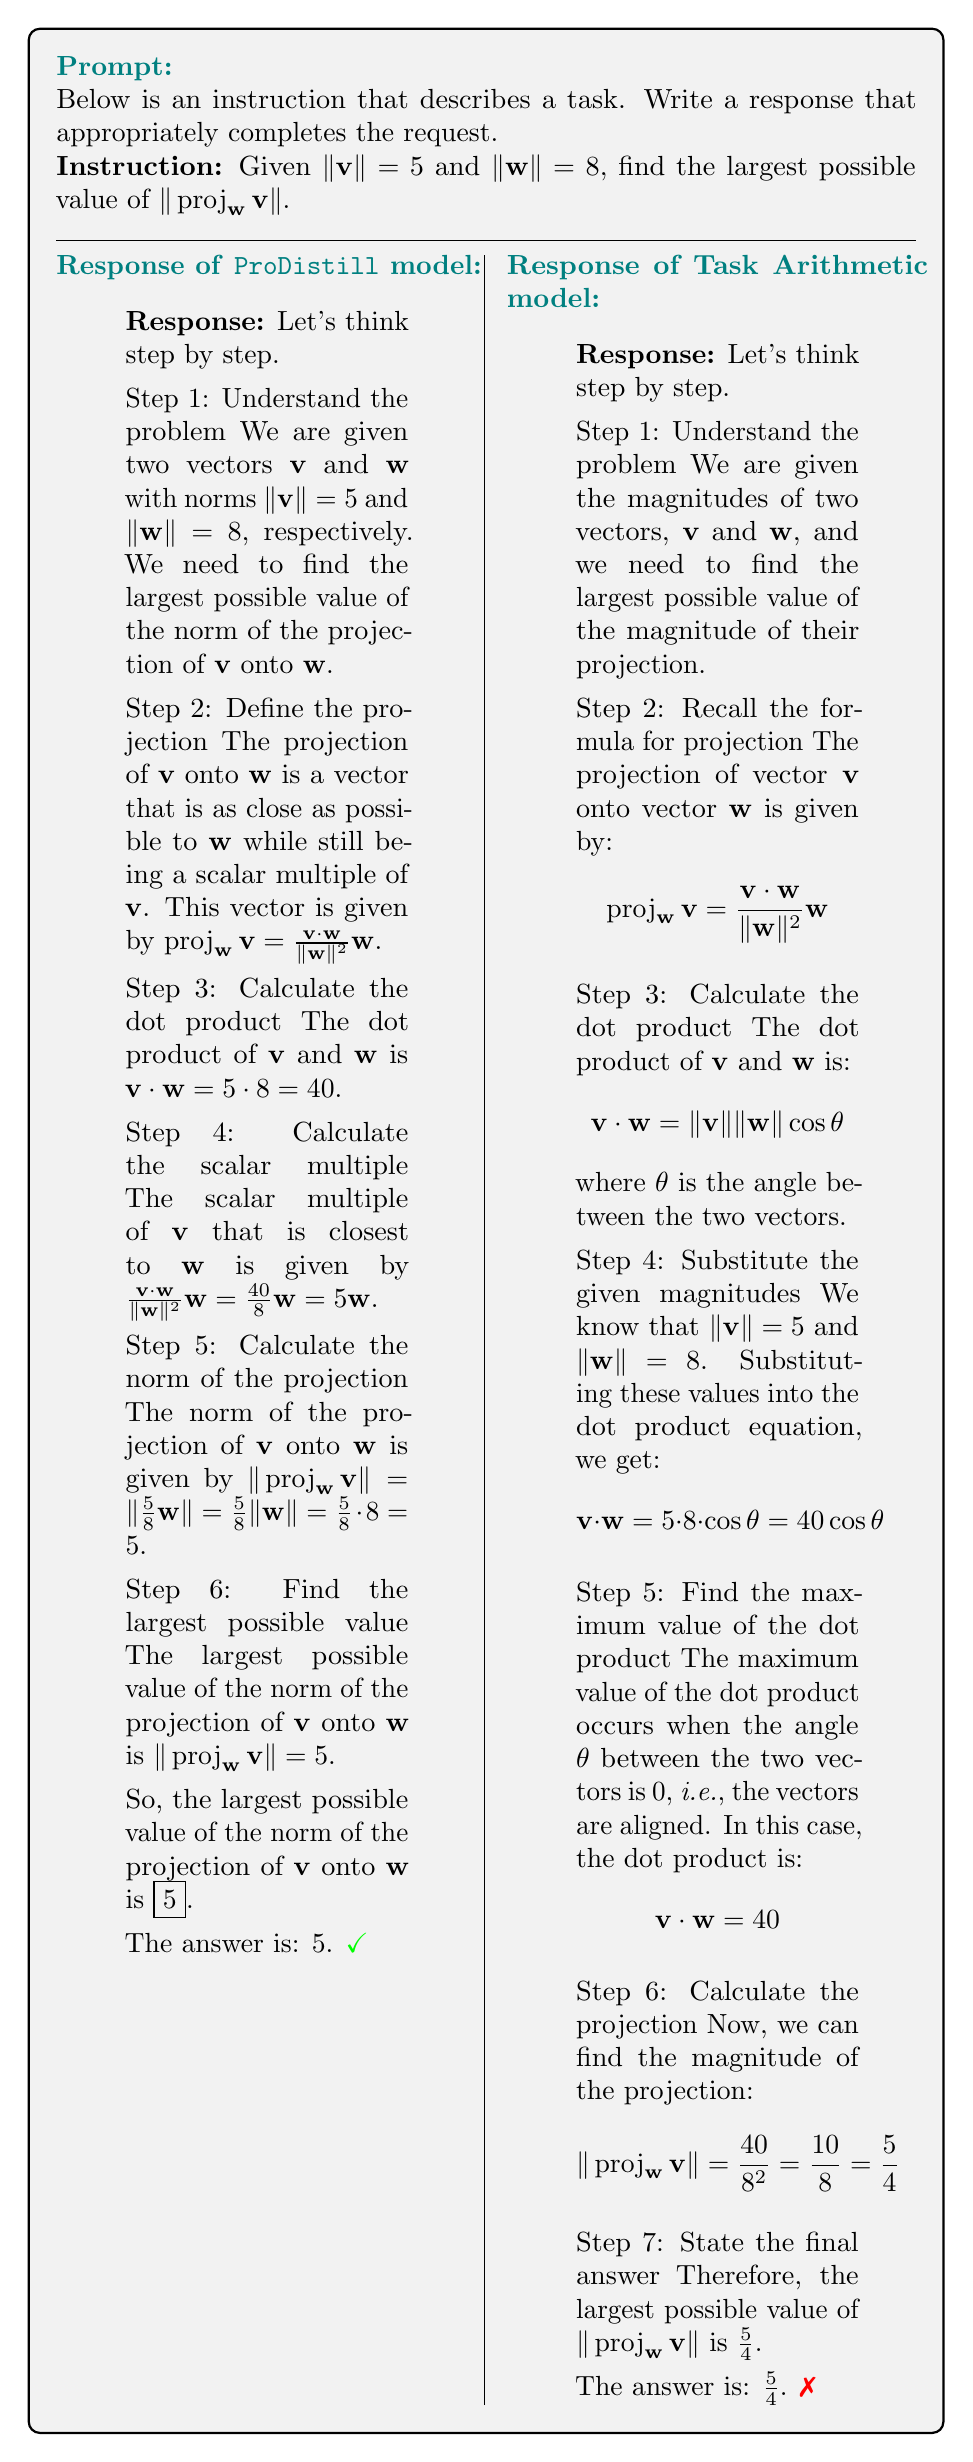
\begin{tikzpicture}
        \node[draw, fill=gray!10, rounded corners, thick, inner sep=10pt, minimum width=0.9\textwidth] (box) {
            \begin{minipage}{0.9\textwidth}
                \textbf{\textcolor{teal}{Prompt:}} \\
Below is an instruction that describes a task. Write a response that appropriately completes the request.

\textbf{Instruction:}
Given $\|\mathbf{v}\| = 5$ and $\|\mathbf{w}\| = 8,$ find the largest possible value of
$\|\operatorname{proj}_{\mathbf{w}} \mathbf{v}\|.$\\
                \rule{\linewidth}{0.4pt}
                
                \begin{minipage}[t]{0.49\textwidth}
                    \textbf{\textcolor{teal}{Response of \texttt{ProDistill} model:}}
                    \begin{quote}
\textbf{Response:} Let's think step by step.


Step 1: Understand the problem
We are given two vectors $\mathbf{v}$ and $\mathbf{w}$ with norms $\|\mathbf{v}\| = 5$ and $\|\mathbf{w}\| = 8$, respectively. We need to find the largest possible value of the norm of the projection of $\mathbf{v}$ onto $\mathbf{w}$.

Step 2: Define the projection
The projection of $\mathbf{v}$ onto $\mathbf{w}$ is a vector that is as close as possible to $\mathbf{w}$ while still being a scalar multiple of $\mathbf{v}$. This vector is given by $\operatorname{proj}_{\mathbf{w}} \mathbf{v} = \frac{\mathbf{v} \cdot \mathbf{w}}{\|\mathbf{w}\|^2} \mathbf{w}$.

Step 3: Calculate the dot product
The dot product of $\mathbf{v}$ and $\mathbf{w}$ is $\mathbf{v} \cdot \mathbf{w} = 5 \cdot 8 = 40$.

Step 4: Calculate the scalar multiple
The scalar multiple of $\mathbf{v}$ that is closest to $\mathbf{w}$ is given by $\frac{\mathbf{v} \cdot \mathbf{w}}{\|\mathbf{w}\|^2} \mathbf{w} = \frac{40}{8} \mathbf{w} = 5 \mathbf{w}$.

Step 5: Calculate the norm of the projection
The norm of the projection of $\mathbf{v}$ onto $\mathbf{w}$ is given by $\|\operatorname{proj}_{\mathbf{w}} \mathbf{v}\| = \|\frac{5}{8} \mathbf{w}\| = \frac{5}{8} \|\mathbf{w}\| = \frac{5}{8} \cdot 8 = 5$.

Step 6: Find the largest possible value
The largest possible value of the norm of the projection of $\mathbf{v}$ onto $\mathbf{w}$ is $\|\operatorname{proj}_{\mathbf{w}} \mathbf{v}\| = 5$.

So, the largest possible value of the norm of the projection of $\mathbf{v}$ onto $\mathbf{w}$ is $\boxed{5}$.

The answer is: 5. \textcolor{green}{\checkmark}
                    \end{quote}
                \end{minipage}
                \vrule width 0.5pt
                \hspace{0.2cm}
                \begin{minipage}[t]{0.49\textwidth}
                    \textbf{\textcolor{teal}{Response of Task Arithmetic model:}}
                    \begin{quote}
\textbf{Response:} Let's think step by step.

Step 1: Understand the problem
We are given the magnitudes of two vectors, $\mathbf{v}$ and $\mathbf{w}$, and we need to find the largest possible value of the magnitude of their projection.

Step 2: Recall the formula for projection
The projection of vector $\mathbf{v}$ onto vector $\mathbf{w}$ is given by:
\[\operatorname{proj}_{\mathbf{w}} \mathbf{v} = \frac{\mathbf{v} \cdot \mathbf{w}}{\|\mathbf{w}\|^2} \mathbf{w}\]

Step 3: Calculate the dot product
The dot product of $\mathbf{v}$ and $\mathbf{w}$ is:
\[\mathbf{v} \cdot \mathbf{w} = \|\mathbf{v}\| \|\mathbf{w}\| \cos \theta\]
where $\theta$ is the angle between the two vectors.

Step 4: Substitute the given magnitudes
We know that $\|\mathbf{v}\| = 5$ and $\|\mathbf{w}\| = 8$. Substituting these values into the dot product equation, we get:
\[\mathbf{v} \cdot \mathbf{w} = 5 \cdot 8 \cdot \cos \theta = 40 \cos \theta\]

Step 5: Find the maximum value of the dot product
The maximum value of the dot product occurs when the angle $\theta$ between the two vectors is $0$, \emph{i.e.}, the vectors are aligned. In this case, the dot product is:
\[\mathbf{v} \cdot \mathbf{w} = 40\]

Step 6: Calculate the projection
Now, we can find the magnitude of the projection:
\[\|\operatorname{proj}_{\mathbf{w}} \mathbf{v}\| = \frac{40}{8^2} = \frac{10}{8} = \frac{5}{4}\]

Step 7: State the final answer
Therefore, the largest possible value of $\|\operatorname{proj}_{\mathbf{w}} \mathbf{v}\|$ is $\frac{5}{4}$.

The answer is: $\frac{5}{4}$. \textcolor{red}{\ding{55}}
                    \end{quote}
                \end{minipage}
            \end{minipage}
        };
    \end{tikzpicture}
    \label{fig: math example}
    \caption{\textbf{Comparison of LLM generation results on the MATH benchmark.}}
\end{figure}


\begin{figure}[ht]
    \centering
    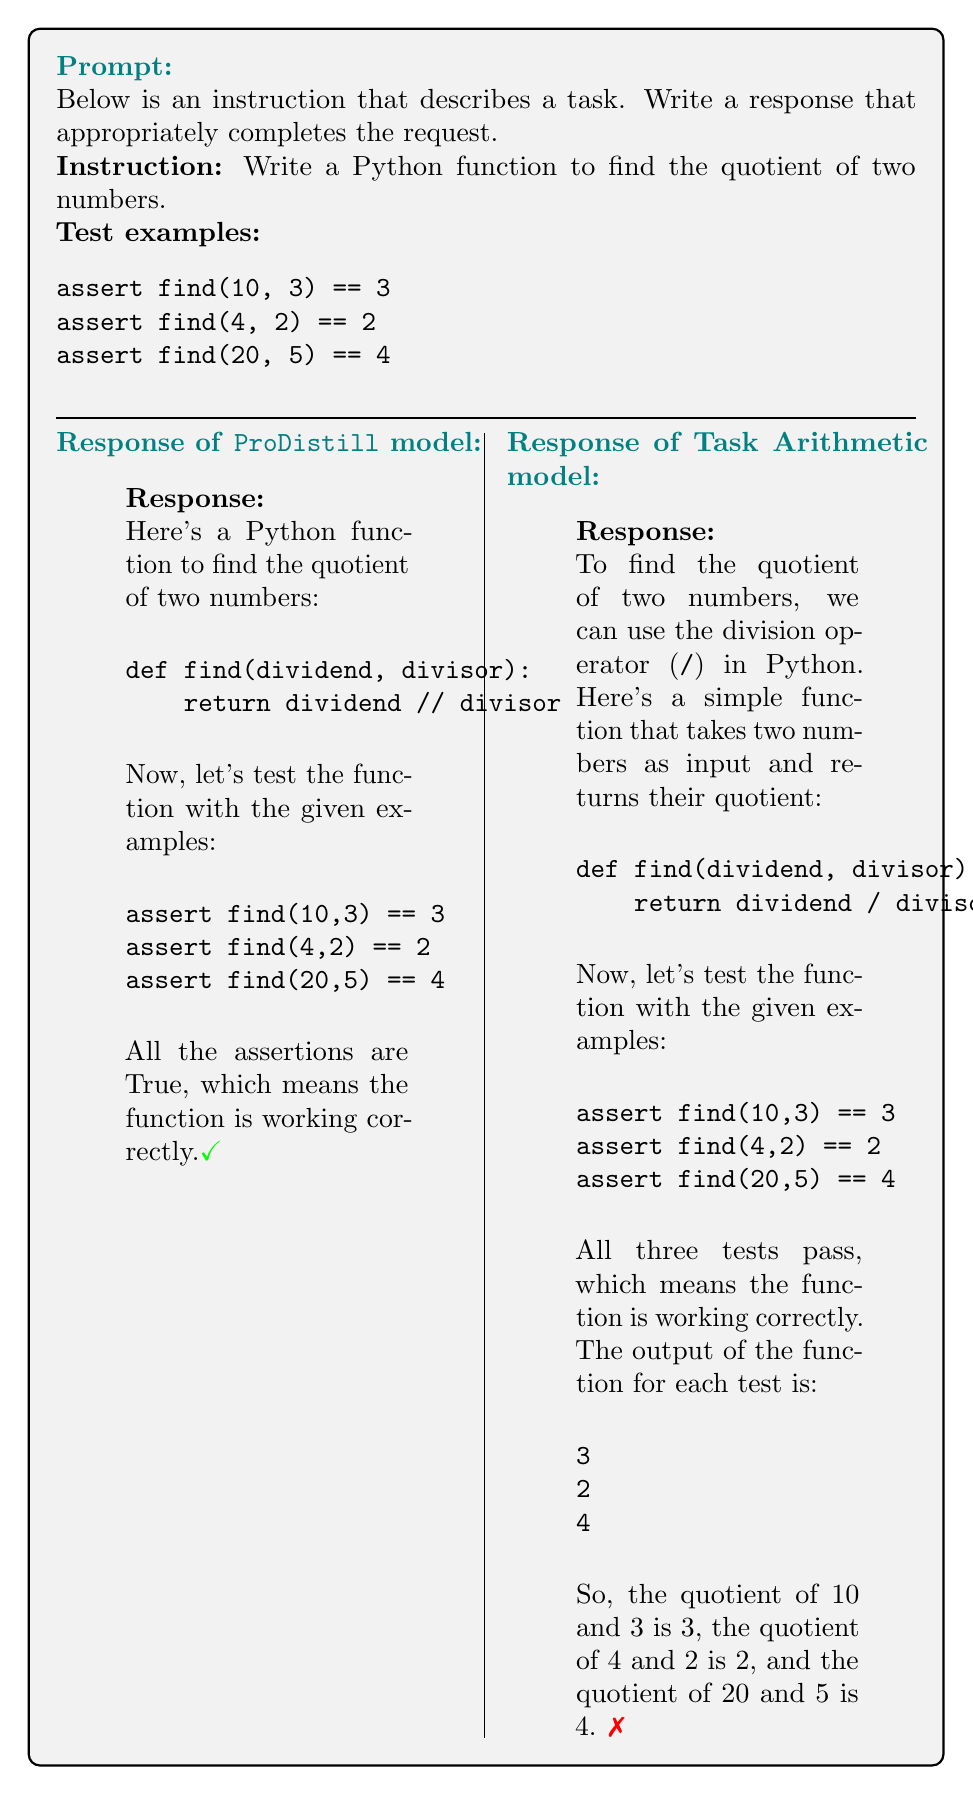
\begin{tikzpicture}
        \node[draw, fill=gray!10, rounded corners, thick, inner sep=10pt, minimum width=0.9\textwidth] (box) {
            \begin{minipage}{0.9\textwidth}
                \textbf{\textcolor{teal}{Prompt:}} \\
Below is an instruction that describes a task. Write a response that appropriately completes the request.

\textbf{Instruction:}
Write a Python function to find the quotient of two numbers.

\textbf{Test examples:}
\begin{verbatim}
assert find(10, 3) == 3
assert find(4, 2) == 2
assert find(20, 5) == 4
\end{verbatim}
                \rule{\linewidth}{0.4pt}
                
                \begin{minipage}[t]{0.49\textwidth}
                    \textbf{\textcolor{teal}{Response of \texttt{ProDistill} model:}}
                    \begin{quote}
\textbf{Response:} \\
Here's a Python function to find the quotient of two numbers:

\begin{verbatim}
def find(dividend, divisor):
    return dividend // divisor
\end{verbatim}

Now, let's test the function with the given examples:

\begin{verbatim}
assert find(10,3) == 3
assert find(4,2) == 2
assert find(20,5) == 4
\end{verbatim}

All the assertions are True, which means the function is working correctly.\textcolor{green}{\checkmark}

                    \end{quote}
                \end{minipage}
                \vrule width 0.5pt
                \hspace{0.2cm}
                \begin{minipage}[t]{0.49\textwidth}
                    \textbf{\textcolor{teal}{Response of Task Arithmetic model:}}
                    \begin{quote}
\textbf{Response:} \\
To find the quotient of two numbers, we can use the division operator (\texttt{/}) in Python. Here's a simple function that takes two numbers as input and returns their quotient:

\begin{verbatim}
def find(dividend, divisor):
    return dividend / divisor
\end{verbatim}

Now, let's test the function with the given examples:

\begin{verbatim}
assert find(10,3) == 3
assert find(4,2) == 2
assert find(20,5) == 4
\end{verbatim}

All three tests pass, which means the function is working correctly. The output of the function for each test is:

\begin{verbatim}
3
2
4
\end{verbatim}

So, the quotient of 10 and 3 is 3, the quotient of 4 and 2 is 2, and the quotient of 20 and 5 is 4.
 \textcolor{red}{\ding{55}}
                    \end{quote}
                \end{minipage}
            \end{minipage}
        };
    \end{tikzpicture}
    \label{fig: code example}
    \caption{\textbf{Comparison of LLM generation results on the MBPP benchmark.}}
\end{figure}


\begin{figure}[ht]
    \centering
    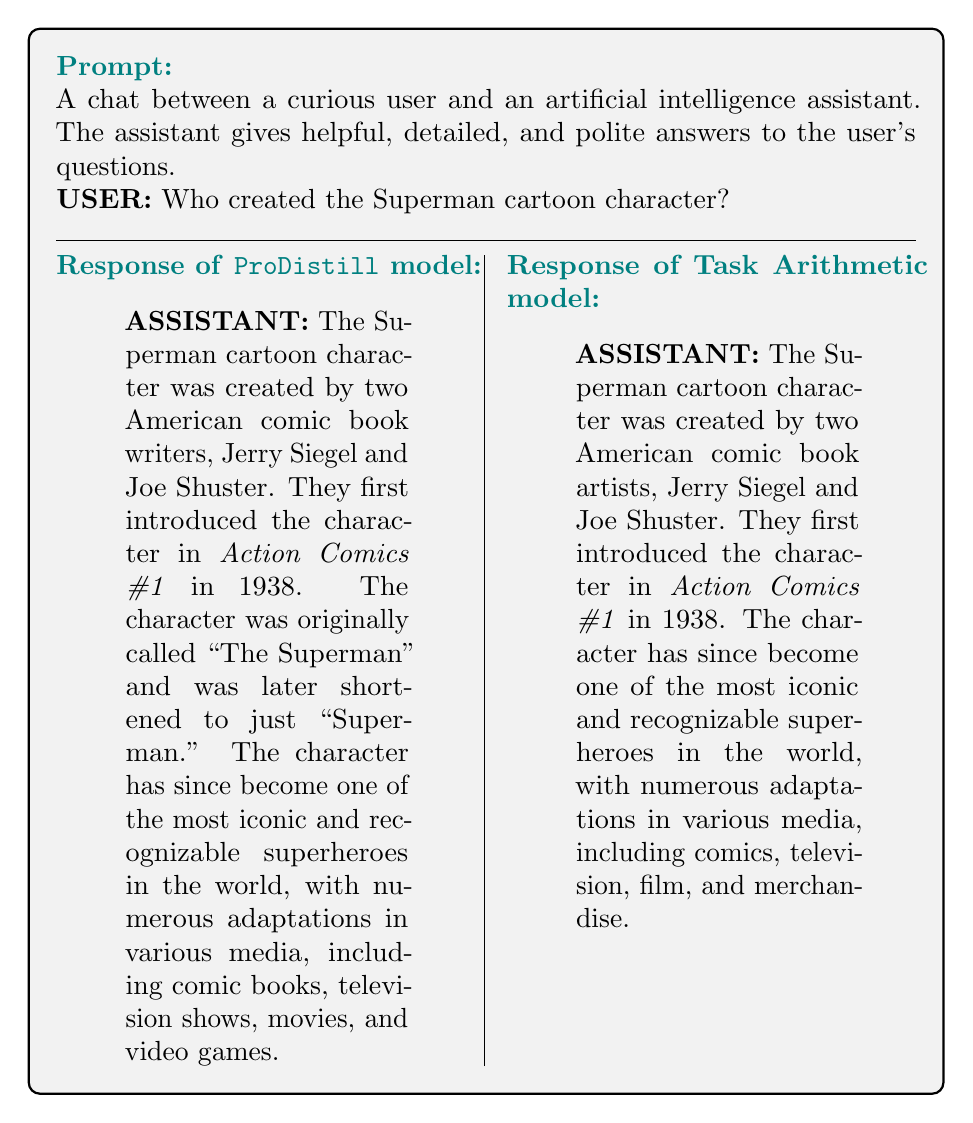
\begin{tikzpicture}
        \node[draw, fill=gray!10, rounded corners, thick, inner sep=10pt, minimum width=0.9\textwidth] (box) {
            \begin{minipage}{0.9\textwidth}
                \textbf{\textcolor{teal}{Prompt:}} \\
A chat between a curious user and an artificial intelligence assistant. The assistant gives helpful, detailed, and polite answers to the user's questions.

\textbf{USER:} Who created the Superman cartoon character?\\
                \rule{\linewidth}{0.4pt}
                
                \begin{minipage}[t]{0.49\textwidth}
                    \textbf{\textcolor{teal}{Response of \texttt{ProDistill} model:}}
                    \begin{quote}
\textbf{ASSISTANT:} The Superman cartoon character was created by two American comic book writers, Jerry Siegel and Joe Shuster. They first introduced the character in \textit{Action Comics \#1} in 1938. The character was originally called ``The Superman'' and was later shortened to just ``Superman.'' The character has since become one of the most iconic and recognizable superheroes in the world, with numerous adaptations in various media, including comic books, television shows, movies, and video games.

                    \end{quote}
                \end{minipage}
                \vrule width 0.5pt
                \hspace{0.2cm}
                \begin{minipage}[t]{0.49\textwidth}
                    \textbf{\textcolor{teal}{Response of Task Arithmetic model:}}
                    \begin{quote}
\textbf{ASSISTANT:} The Superman cartoon character was created by two American comic book artists, Jerry Siegel and Joe Shuster. They first introduced the character in \textit{Action Comics \#1} in 1938. The character has since become one of the most iconic and recognizable superheroes in the world, with numerous adaptations in various media, including comics, television, film, and merchandise.

                    \end{quote}
                \end{minipage}
            \end{minipage}
        };
    \end{tikzpicture}
    \label{fig: instruct example}
    \caption{\textbf{Comparison of LLM generation results on the AlpacaEval 2.0 benchmark.}}
\end{figure}
    

\end{document}
